\section{Planeación de rutas}

\begin{frame}\frametitle{Planeación de movimientos}
  El problema de la planeación de movimientos comprende cuatro tareas principales:
  \begin{itemize}
  \item Navegación: encontrar un conjunto de puntos $q \in Q_{free}$ que permitan al robot moverse desde una configuración inicial $q_{start}$ a una configuración final $q_{goal}$. 
  \item Mapeo: construir una representación del ambiente a partir de las lecuras de los sensores y la trayectoria del robot. 
  \item Localización: determinar la configuración $q$ dado un mapa y lecturas de los sensores. 
  \item Barrido: pasar un actuador por todos los puntos $q\in Q_b \subset Q$.
  \end{itemize}
\end{frame}

\begin{frame}\frametitle{Representación del ambiente}
  Un mapa es cualquier representación del ambiente útil en la toma de decisiones.
  \begin{itemize}
  \item Interiores (se suelen representar en 2D)
    \begin{itemize}
    \item Celdas de ocupación
    \item Mapas de líneas
    \item Mapas topológicos: Diagramas de Voronoi generalizados. 
    \item Mapas basados en \textit{Landmarks}
    \end{itemize}
  \item Exteriores (suelen requerir una representación 3D)
    \begin{itemize}
    \item Celdas de elevación
    \item Celdas de ocupación 3D
    \item Octomaps
    \end{itemize}
  \end{itemize}
\end{frame}

\begin{frame}\frametitle{Celdas de ocupación}
  Es un tipo de mapa geométrico. El espacio se discretiza con una resolución determinada y a cada celda se le asigna un número $p\in[0,1]$ que indica su nivel de ocupación. En un enfoque probabilístico este número se puede interpretar como la certeza que se tiene de que una celda esté ocupada.
  \begin{figure}
    \centering
    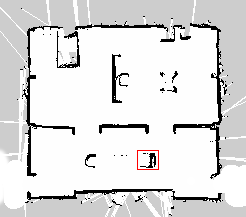
\includegraphics[width=0.4\textwidth]{Figures/OccupancyGrid.png}
    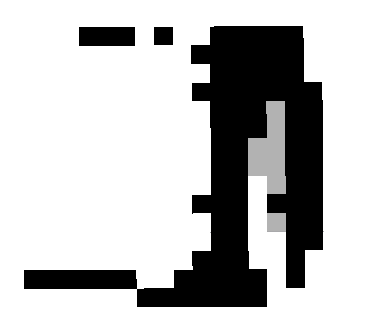
\includegraphics[width=0.4\textwidth]{Figures/UniversumZoom.png}
    \end{figure}
  El mapa resultante se representa en memoria mediante una matriz de valores de ocupación. En ROS, los mapas utilizan el mensaje \texttt{nav\_msgs/OccupancyGrid}.
\end{frame}

\begin{frame}\frametitle{Inflado de celdas de ocupación}
  Aunque las celdas de ocupación representan el espacio donde hay obstáculos y donde no, en realidad, el robot no puede posicionarse en todas las celdas libres, debido a su tamaño, como se observa en la figura:
  \begin{columns}
    \begin{column}{0.6\textwidth}
      \begin{figure}
        \centering
        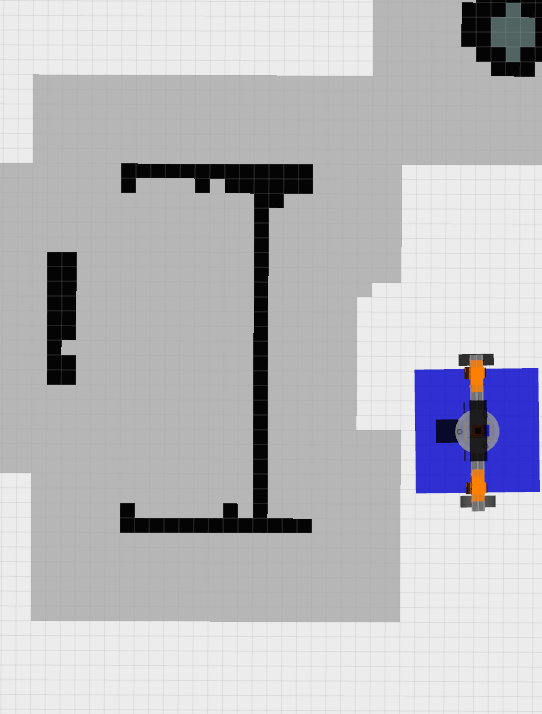
\includegraphics[width=0.45\textwidth]{Figures/InflationExample1.png}
        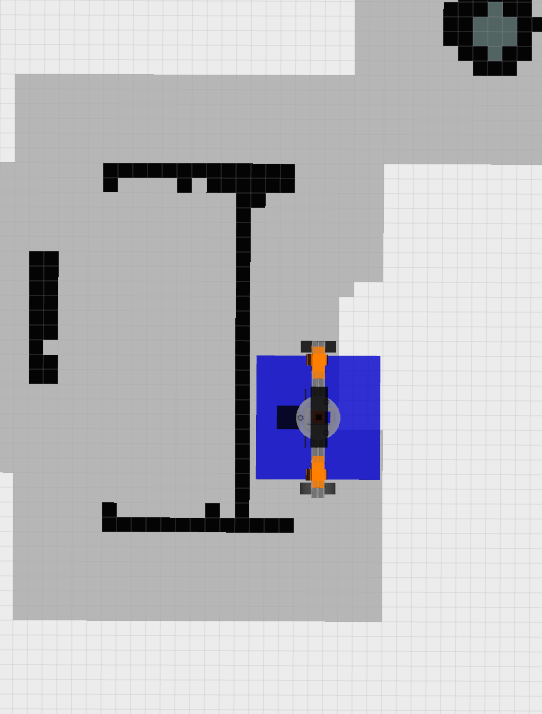
\includegraphics[width=0.45\textwidth]{Figures/InflationExample2.png}
      \end{figure}
    \end{column}
    \begin{column}{0.4\textwidth}
      \begin{itemize}
      \item Celdas blancas: espacio libre.
      \item Celdas negras: espacio con obstáculos.
      \item Celdas grises: espacio sin obstáculos donde el robot no puede estar debido a su tamaño. 
      \end{itemize}
    \end{column}
  \end{columns}
  \begin{itemize}
  \item Un mapa de celdas de ocupación debe \textit{inflarse} antes de usarse para planear rutas.
  \item Esta operación se conoce como \textit{dilatación} y es un operador morfológico como se verá en la sección de conceptos de visión.
  \item El inflado se usa para planeación de rutas, no para localización.
  \end{itemize}
\end{frame}

\begin{frame}\frametitle{Inflado de celdas de ocupación}
  \label{fr:inflation}
  \begin{algorithm}[H]
    \DontPrintSemicolon
    \KwData {\;
      Mapa $M$ de celdas de ocupación\;
      Radio de inflado $r_i$
    }
    \KwResult{Mapa inflado $M_{inf}$}
    $M_{inf} = $ Copia de $M$\;
    \ForEach{$i\in [0,\dots,rows)$}
      {
        \ForEach{$j\in [0,\dots,cols)$}
          {
            //Si la celda está ocupada, marcar como ocupadas las $r_i$ celdas de alrededor.\;
            \If{$M[i,j] == 100$ }
               {
                 \ForEach{$k_1\in [-r_i,\dots,r_i]$}
                   {
                     \ForEach{$k_2\in [-r_i,\dots,r_i]$}
                       {
                         $M_{inf}[i+k_1, j+k_2] = 100$
                       }
                   }
               }    
          }
        }
        \label{alg:inflation}
        \caption{Algoritmo de inflado de mapas}
  \end{algorithm}
\end{frame}

\begin{frame}\frametitle{Mapas de líneas}
  También son mapas geométricos, pero al almancenar \textit{features} requieren mucho menos memoria. La desventaja es la dificultad para extraer líneas del ambiente y la poca precisión en el empatado. 
  \begin{figure}
    \centering
    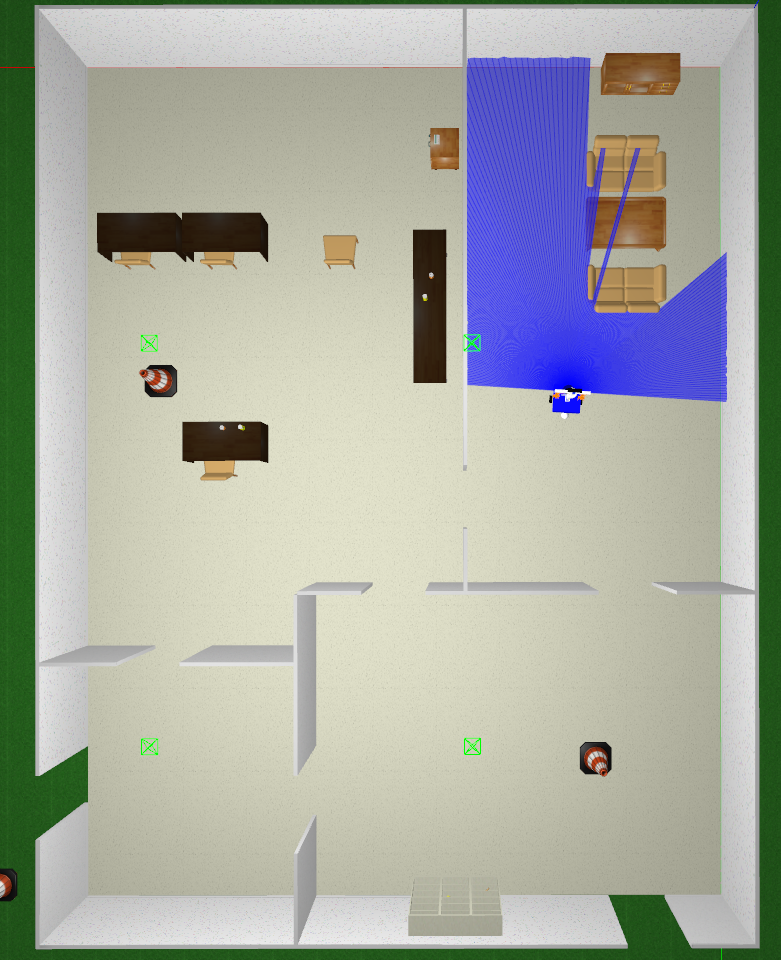
\includegraphics[width=0.3\textwidth]{Figures/MapLinesGazebo.png}
    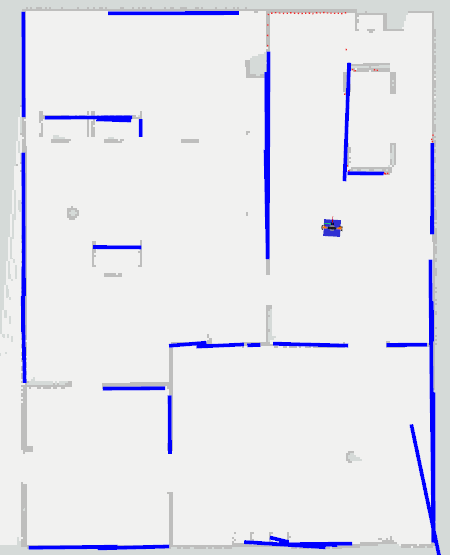
\includegraphics[width=0.3\textwidth]{Figures/MapLines.png}
  \end{figure}
  Algunos métodos para extraer líneas:
  \begin{itemize}
  \item \textit{Split and merge}
  \item Transformada Hough (se verá en la sección de visión computacional)
  \item RANSAC
  \end{itemize}
\end{frame}

\begin{frame}\frametitle{Algoritmo \textit{Split and Merge}}
  Se utiliza principalmente cuando los datos provienen de un sensor Lidar y por lo tanto, los puntos están en secuencia.
  \[\]
  \begin{columns}
    \begin{column}{0.65\textwidth}
      \begin{algorithm}[H]
        \DontPrintSemicolon
        \KwData {Conjunto de puntos $P$}
        \KwResult{Conjunto de líneas en forma normal $(\rho, \theta$)}
        \;
        Ajustar una recta $L$ al conjunto $P$ por mínimos cuadrados\;
        Encontrar el punto $p_i$ más lejano a la recta\;
          \uIf{$d(p_i, L) > d_{0}$}
             {
               Dividir $P$ en dos subconjuntos $P_1$ y $P_2$ usando $p_i$ como pivote\;
               Aplicar este algoritmo recursivamente para $P_1$ y $P_2$\;
               Devolver las rectas de ambos subconjuntos
             }
             \Else
                 {
                   Devolver la recta $L$ en forma normal $(\rho, \theta)$\;
                 }
                 \caption{\textit{Split}}
        \end{algorithm}
    \end{column}
    \begin{column}{0.35\textwidth}
      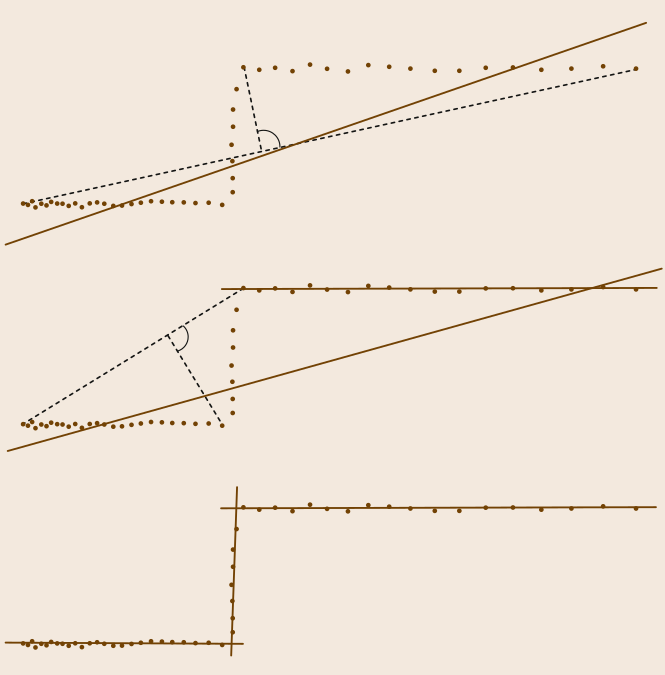
\includegraphics[width=\textwidth]{Figures/SplitAndMerge.png}
    \end{column}
  \end{columns}
\end{frame}

\begin{frame}\frametitle{Algoritmo \textit{Split and Merge}}
  \label{fr:split_merge}
  El algoritmo anterior realiza la partición (\textit{split}) del conjunto de puntos en posibles rectas y obtiene la ecuación para cada conjunto por mínimos cuadrados. La etapa de mezcla (\textit{merge}) consiste simplemente en considerar como una sola recta, dos segmentos con parámetros $(\rho, \theta)$ similares. Los parámetros a sintonizar en este algoritmo son:
  \begin{itemize}
  \item $d_0$ : umbral de distancia entre un punto $p_i$ y la recta $L$
  \item $N_{min}$ : número mínimo de puntos para considerar que un subconjunto puede ser una recta.
  \item $\rho_{tol}$ : valor máximo de diferencia entre dos rectas con $\rho_1$ y $\rho_2$ para considerarlas como una sola recta.
  \item $\theta_{tol}$ : valor máximo de diferencia entre dos rectas con $\theta_1$ y $\theta_2$ para considerarlas como una sola recta. 
  \end{itemize}
\end{frame}

\begin{frame}\frametitle{Mínimos cuadrados}
  Este método busca minimizar las distancias entre los puntos $(x_i,y_i)$ y la recta en forma normal dada por los parámetros $(\rho, \theta)$.
  \[\]
  Dado un conjunto de puntos $(x_i, y_i)$, la recta $(\rho,\theta)$ que mejor se ajusta se puede obtener con:
  \begin{eqnarray*}
    \theta &=& \frac{1}{2}\atantwo\left(-2\sum_i (\bar{x} - x_i)(\bar{y}-y_i)\quad,\quad \sum_i\left[(\bar{y} - y_i)^2 - (\bar{x} - x_i)^2\right]\right)\\
    \rho &=& \bar{x}\cos\theta + \bar{y}\sin\theta
  \end{eqnarray*}
  con
  \begin{eqnarray*}
    \bar{x} &=& \frac{1}{n}\sum_i x_i\\
    \bar{y} &=& \frac{1}{n}\sum_i y_i
  \end{eqnarray*}
\end{frame}

\begin{frame}\frametitle{Diagrama de Voronoi Generalizado}
  \begin{itemize}
  \item A diferencia de los mapas geométricos, donde se busca reflejar la forma exacta del ambiente, los \textbf{mapas topológicos} buscan representar solo las relaciones espaciales de los puntos de interés.
  \item Los Diagramas de Voronoi dividen el espacio en regiones. Cada región está asociada a un punto llamado semilla, sitio o generador. Una región asociada a una semilla $x$ contiene todos los puntos $p$ tales que $d(x,p)$ es menor o igual que la distancia $d(x^\prime, p)$ a cualquier otra semilla $x^\prime$.
  \item Un diagrama de Voronoi generalizdo (GVD) considera que las semillas pueden ser objetos con dimensiones y no solo puntos. 
  \end{itemize}
  \begin{figure}
    \centering
    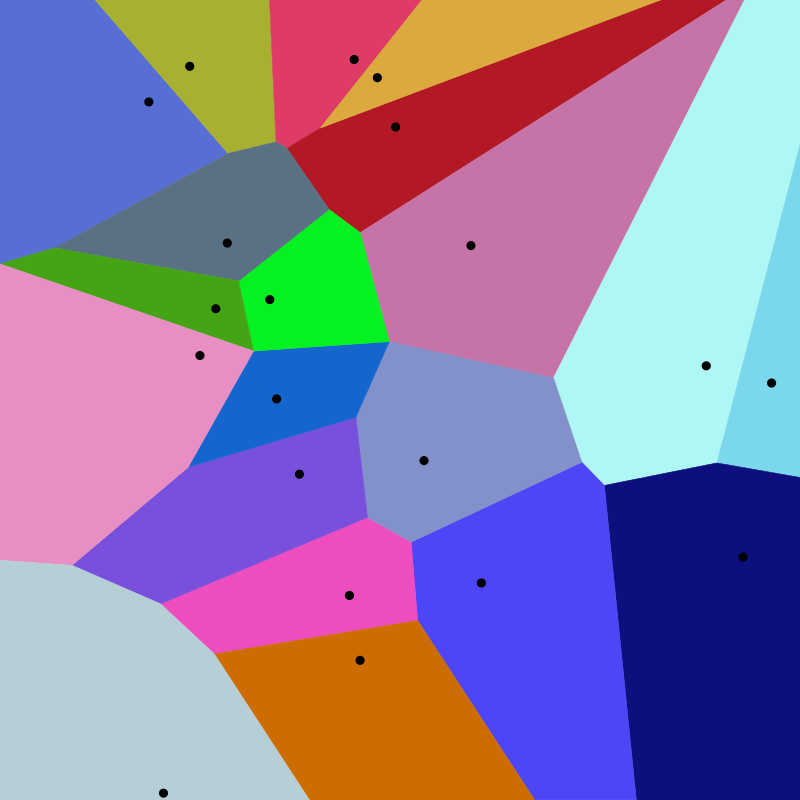
\includegraphics[height=0.4\textheight]{Figures/GVD.png}
    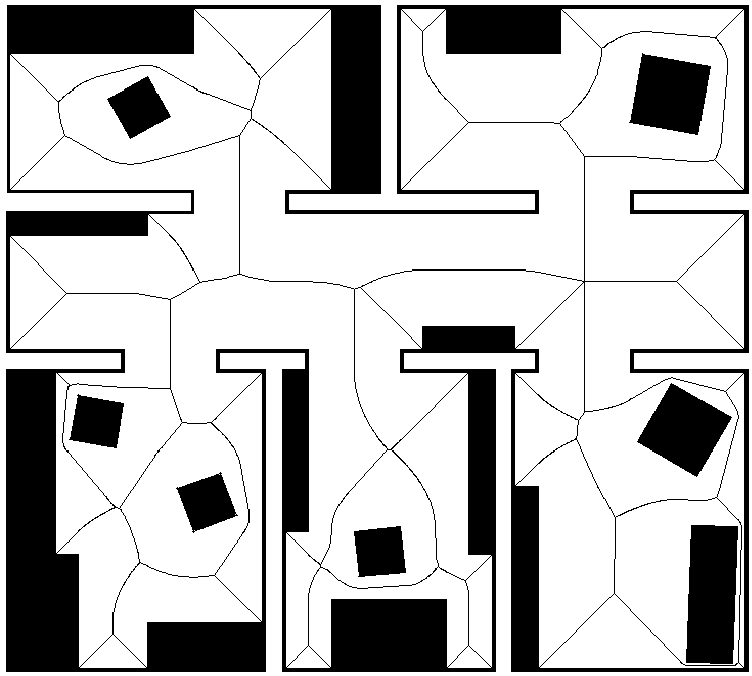
\includegraphics[height=0.4\textheight]{Figures/GVDExample.png}
  \end{figure}
  \begin{itemize}
    \item La forma de las regiones depende de la función de distancia que se utilice. 
  \end{itemize}
\end{frame}

\begin{frame}\frametitle{El algoritmo \textit{Brushfire}}
  \begin{columns}
    \begin{column}{0.65\textwidth}
      \begin{itemize}
      \item Obtener un GVD es aún un problema abierto
      \item Se simplifica el problema si se asume que el espacio está representado por Celdas de Ocupación
      \item En este caso el GVD se puede obtener mediante el algoritmo \textit{Brushfire}
      \item El mapa de rutas mostrado en la figura se forma con las celdas que son máximos locales en el mapa de distancias devuelto por Brushfire, es decir, son las celdas que son fronteras entre las regiones de Voronoi.
      \item Estas celdas también son aquellas equidistantes a los dos obstáculos más cercanos. 
      \end{itemize}
    \end{column}
    \begin{column}{0.35\textwidth}
      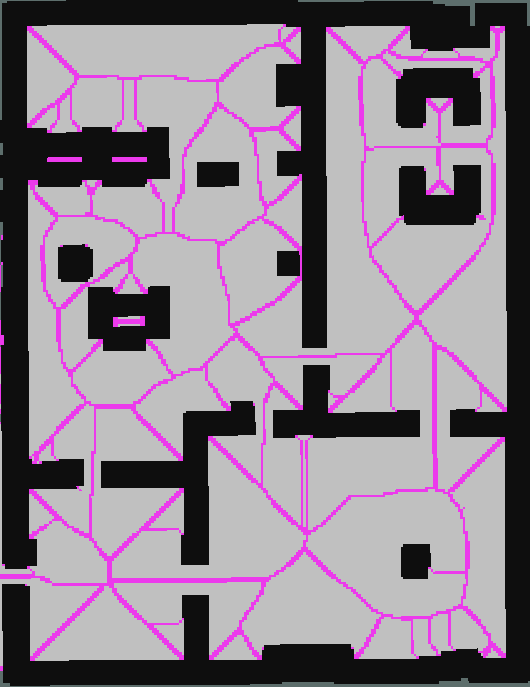
\includegraphics[width=\textwidth]{Figures/GVDFromGrid.png}
    \end{column}
  \end{columns}
\end{frame}

\begin{frame}\frametitle{El algoritmo \textit{Brushfire}}
  \begin{columns}
    \begin{column}{0.65\textwidth}
      \begin{algorithm}[H]
        \DontPrintSemicolon
        \KwData {Mapa de celdas de ocupación $M$}
        \KwResult{Distancias de cada celda al objeto más cercano}
        \;
        Fijar $d(p) = 0$ para toda celda $p$ en los obstáculos\;
        Fijar $d(p) = -1$ para toda celda $p$ en el espacio libre\;
        Crear una cola $Q$ y agregar toda $p$ en los obstáculos\;
        \While{$Q$ no esté vacía}
              {
                $x = $ desencolar de Q\;
                \ForAll{celdas $p$ vecinas de $x$}
                       {
                         \uIf{$d(p) == -1$}
                            {
                              Agregar $p$ a $Q$\;
                              Fijar $d(p) = x + d(p,x)$\;
                            }
                            \Else
                                {
                                  Fijar $d(p) = min(d(p), x+d(p,x))$
                                }
                       }
              }
        \caption{Brushfire}
        \end{algorithm}
    \end{column}
    \begin{column}{0.35\textwidth}
      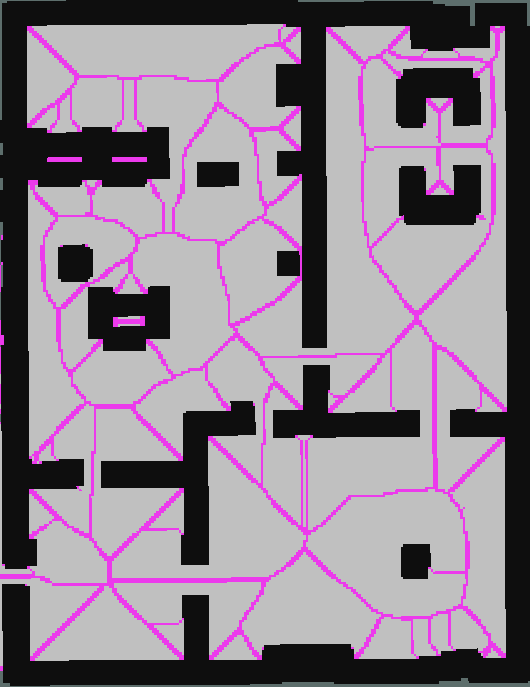
\includegraphics[width=\textwidth]{Figures/GVDFromGrid.png}
    \end{column}
  \end{columns}
\end{frame}


\begin{frame}[containsverbatim]\frametitle{Ejercicio 2 - Representación del ambiente}
  \begin{enumerate}
  \item Abra el archivo \texttt{catkin\_ws/src/students/scripts/assignment02a.py} e implemente el algoritmo de inflado de mapas (algoritmo \ref{alg:inflation}, diapositiva \ref{fr:inflation})
  \item Abra una terminal y corra la simulación con el comando (revise las instrucciones en el README del repositorio):
\begin{verbatim}
 roslaunch bring_up path_planning.launch
\end{verbatim}
  \item En otra terminal, corra el ejercicio 2a con el comando:
\begin{verbatim}
 rosrun students assignment02a.py _inflation_radius:=0.2
\end{verbatim}
  \item Obseve lo que sucede en el visualizador RViz.
  \item Detenga la práctica y ejecútela de nuevo con radios de inflado diferentes, por ejemplo:
\begin{verbatim}
 rosrun students assignment02a.py _inflation_radius:=0.3
\end{verbatim}
Observe qué sucede. ¿Qué pasa si el radio de inflado es muy grande o muy pequeño?
  \item En otra terminal, corra el algoritmo \textit{split and merge} con el comando:
\begin{verbatim}
 rosrun students assignment02b.py _dist:=0.01 _points:=3 _rho:=0.05 _theta:=0.05
\end{verbatim}
\item Detenga la detección de líneas y ejecútela nuevamente con diferentes parámetros de sintonización. Con la GUI, mueva el robot a diferentes puntos del mapa para verificar la correcta sintonización de dicho parámetros.
  \end{enumerate}
\end{frame}

\begin{frame}[containsverbatim]\frametitle{Ejercicio 2 - Representación del ambiente}
    \begin{enumerate}
    \setcounter{enumi}{7}
  \item En otra terminal, corra el algoritmo \textit{Brushfire} para obtener un Diagrama de Voronoi Generalizado a partir del mapa inflado (el ejercicio 02a debe estar corriendo):
\begin{verbatim}
 rosrun students assignment02c.py
\end{verbatim}

  \item Detenga el GVD y abra el archivo \texttt{catkin\_ws/src/students/scripts/assignment02c.py} y en las líneas 54 y 57 cambie la distancia Euclideana por distancia de Manhattan (revise los comentarios arriba de cada línea).
  \item Ejecute nuevamente la obtención del GVD y observe lo que sucede en el visualizador RViz
  \end{enumerate}
\end{frame}


\begin{frame}\frametitle{Planeación de rutas}
  La planeación de rutas consiste en encontrar una secuencia de puntos $q\in Q_{free}$ que permitan al robot moverse desde una configuración inicial $q_{start}$ hasta una configuración final $q_{goal}$.
  \begin{itemize}
  \item Una \textbf{ruta} es solo la secuencia de configuraciones para llegar a la meta.
  \item Cuando la secuencia de configuraciones se expresa en función del tiempo, entonces se tiene una \textbf{trayectoria}. 
  \end{itemize}
  En este curso solo vamos a hacer planeación de rutas, no de trayectorias (para navegación).\\
  Existen varios métodos para planear rutas. La mayoría de ellos se pueden agrupar en:
  \begin{itemize}
  \item Métodos basados en muestreo
  \item Métodos basados en grafos
  \end{itemize}
\end{frame}

\begin{frame}\frametitle{Métodos basados muestreo}
  Como su nombre lo indica, consisten en tomar muestras aleatorias del espacio libre. Si es posible llegar en línea recta de la configuración actual al punto muestrado, entonces se agrega a la ruta.
  Ejemplos:
  \begin{itemize}
  \item RRT (Rapidly-exploring Random Trees)
  \item RRT-Bidireccional
  \item RRT-Extendido
  \end{itemize}
\end{frame}

\begin{frame}\frametitle{\textit{Rapidly-exploring Random Trees}}
  Consiste en construir un árbol a partir de muestras aleatorias del espacio libre.
  \begin{columns}
    \begin{column}{0.4\textwidth}
      \begin{algorithm}[H]\small
        \KwData{Mapa, $q_{s} = $ Punto origen }
        \KwResult{Espacio explorado}
        Árbol[0] = $q_{s}$\;
        $k$ = 0\;
        \While{$k < k_{max}$ }
              {
                $q_{r}$ = ConfiguracionAleaoria()\;
                Extiende(Árbol, $q_{r}$)\;
                $k++$\;
              }
              \Return Árbol\;
              \caption{RRT}
      \end{algorithm}
    \end{column}
    \begin{column}{0.6\textwidth}
      \begin{figure}
        \centering
        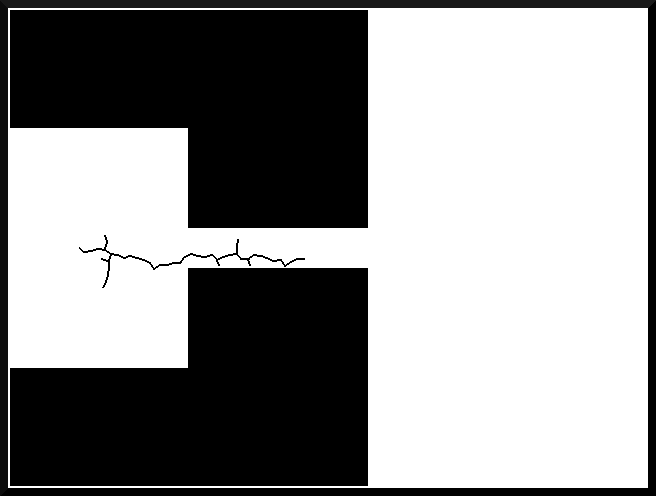
\includegraphics[width=0.45\textwidth]{Figures/RRTO010.png}
        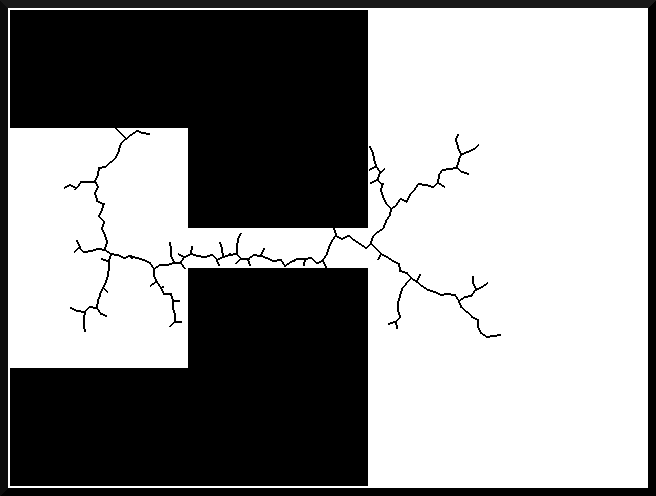
\includegraphics[width=0.45\textwidth]{Figures/RRTO0100.png}
        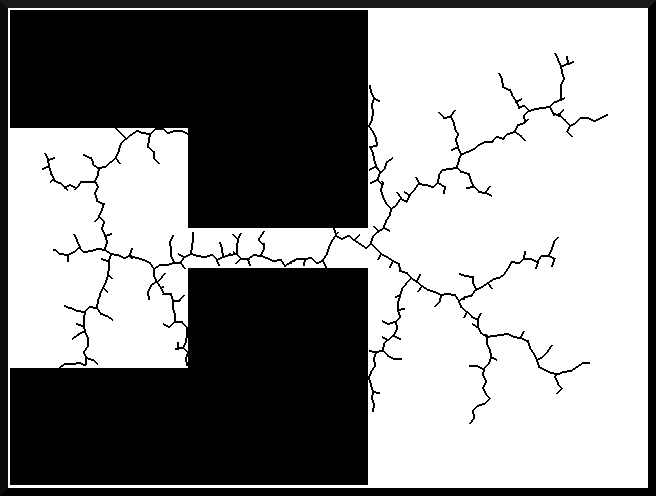
\includegraphics[width=0.45\textwidth]{Figures/RRTO0300.png}
      \end{figure}
    \end{column}
  \end{columns}
\end{frame}

\begin{frame}\frametitle{Métodos basados en grafos}
  Estos métodos consideran el ambiente como un grafo. En el caso de celdas de ocupación, cada celda libre es un nodo que está conectado con las celdas vecinas que también estén libres. Los pasos generales de este tipo de algorimos se pueden resumir en:
  \[\]
  \begin{algorithm}[H]
    \footnotesize
    \DontPrintSemicolon
    \KwData {Mapa $M$ de celdas de ocupación, configuración inicial $q_{start}$, configuración meta $q_{goal}$}
    \KwResult{Ruta $P=[q_{start},q_1, q_2, \dots , q_{goal}]$}
    Obtener los nodos $n_s$ y $n_g$ correspondientes a $q_{start}$ y $q_{goal}$\;
    Lista abierta $OL = \emptyset$ y lista cerrada $CL = \emptyset$\;
    Agregar $n_s$ a $OL$\;
    Nodo actual $n_c = n_s$\;
    \While{$OL\neq \emptyset$ y $n_c\neq n_g$}
    {
      Seleccionar $n_c$ de $OL$ \textbf{bajo algún criterio}\;
      Agregar $n_c$ a $CL$\;
      Expandir $n_c$\;
      Agregar a $OL$ los vecinos de $n_c$ que no estén ya en $OL$ ni en $CL$\;
    }
    \If{$n_c\neq n_g$}{Anunciar Falla}
    Obtener la configuración $q_i$ para cada nodo $n_i$ de la ruta\;
  \end{algorithm}
\end{frame}

\begin{frame}\frametitle{Métodos basados en grafos}
  El criterio para seleccinar el siguiente nodo a expandir $n_c$ de la lista abierta, determina el tipo de algoritmo:
  \begin{itemize}
  \item Criterio FIFO: Búsqueda a lo ancho BFS (la lista abierta es una cola)
  \item Criterio LIFO:  Búsqueda en profundidad DFS (la lista abierta es una pila)
  \item Menor valor $g$: Dijkstra (la lista abierta es una cola con prioridad)
  \item Menor valor $f$: A* (la lista abierta es una cola con prioridad)
  \end{itemize}
  Si el costo $g$ para ir de una celda a otra es siempre 1, entonces Dijkstra es equivalente a BFS. \\
  A* y Dijkstra siempre calculan la misma ruta pero A* lo hace más rápido. 
\end{frame}

\begin{frame}\frametitle{Mapas de costo}
  \begin{itemize}
  \item Los métodos como Dijkstra y A* minimizan una función de costo. Esta función podría ser distancia, tiempo de recorrido, número de vuelta, energía gastada, entre otras.
  \item En este curso se empleará como costo una combinación de distancia recorrida más peligro de colisión (cercanía a los obstáculos).
  \item De este modo, las rutas serán un equilibrio entre rutas cortas y rutas seguras.
  \end{itemize}
  \begin{figure}
    \centering
    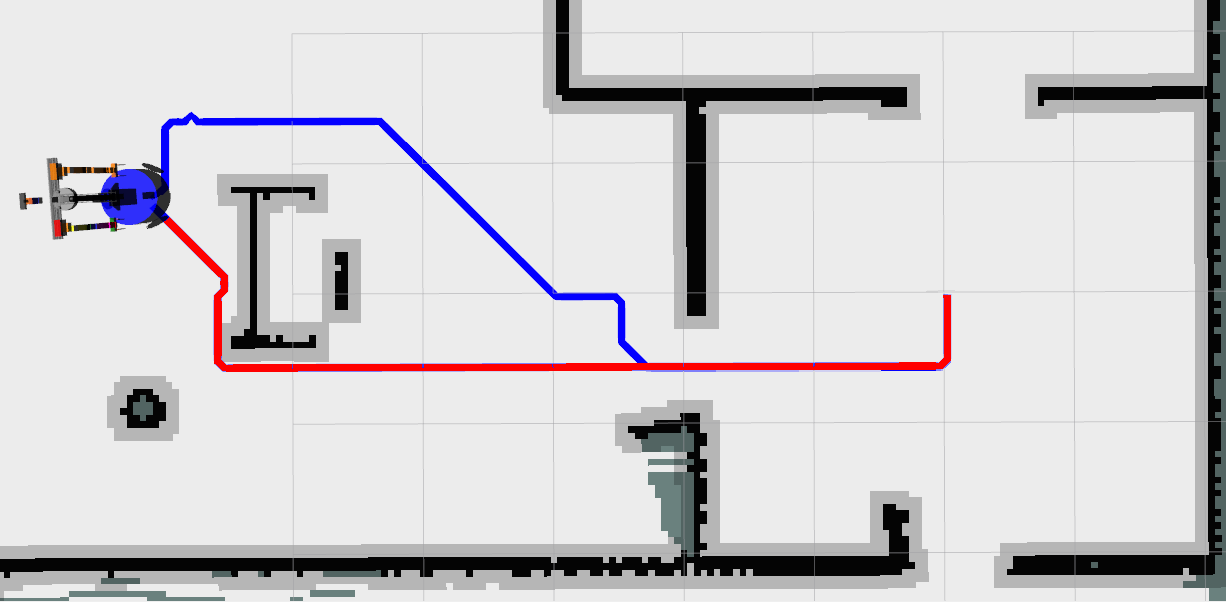
\includegraphics[width=0.5\textwidth]{Figures/AStarComparison.png}
  \end{figure}
\end{frame}

\begin{frame}\frametitle{Mapas de costo}
  \begin{itemize}
  \item Se utilizará como costo una función de \textit{cercanía}.
  \item Se calcula de forma similar al algoritmo Brushfire, pero la función decrece conforme nos alejamos de los objetos. 
  \end{itemize}
  \begin{columns}
    \begin{column}{0.6\textwidth}
      \begin{algorithm}[H]
        \footnotesize
        \DontPrintSemicolon
        \KwData {\;
          Mapa $M$ de celdas de ocupación\;
          Radio de costo $r_c$
        }
        \KwResult{Mapa de costo $M_c$}
        \;
        $M_c = $ Copia de $M$\;
        \ForEach{$i\in [0,\dots,rows)$}
          {
            \ForEach{$j\in [0,\dots,cols)$}
              {
                //Si está ocupada, calcular el costo de $r_c$ celdas alrededor.\;
                \If{$M[i,j] == 100$ }
                   {
                     \ForEach{$k_1\in [-r_c,\dots,r_c]$}
                             {
                               \ForEach{$k_2\in [-r_c,\dots,r_c]$}
                                       {
                                         $C = r_c - max(|k1|,|k2|) + 1$\;
			                 $M_c[i+k1,j+k2] = max(C, M_c[i+k1,j+k2]$\;
                                       }
                             }
                   }    
              }
            }
            \caption{Mapa de costo}
      \end{algorithm}
    \end{column}
    \begin{column}{0.4\textwidth}
      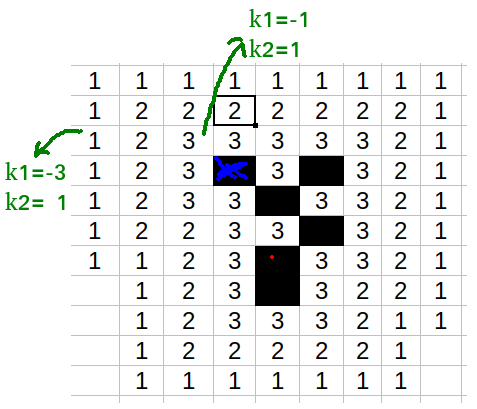
\includegraphics[width=0.95\textwidth]{Figures/CostMap.png}
    \end{column}
  \end{columns}
\end{frame}


\begin{frame}\frametitle{El algoritmo A*}
  \begin{itemize}
  \item Es un algoritmo completo, es decir, si la ruta existe, seguro la encontrará, y si no existe, lo indicará en tiempo finito.
  \item Al igual que Dijkstra, A* encuentra una ruta que minimiza una función de costo, es decir, es un algoritmo óptimo.
  \item Es un algoritmo del tipo de búsqueda informada, es decir, utiliza información sobre el estimado del costo restante para llegar a la meta para priorizar la expansión de ciertos nodos. 
  \item El nodo a expandir se selecciona de acuerdo con la función:
    \[f(n) = g(n) + h(n)\]
    donde
    \begin{itemize}
    \item $g(n)$ es el costo acumulado del nodo $n$
    \item $h(n)$ es una función heurística que \textbf{subestima} el costo de llegar del nodo $n$ al nodo meta $n_g$. 
    \end{itemize}
  \item Se tienen los siguientes conjuntos importantes:
    \begin{itemize}
    \item Lista abierta: conjunto de todos los nodos en la frontera (visitados pero no conocidos). Es una cola con prioridad donde los elementos son los nodos y la prioridad es el valor $f(n)$.
    \item Lista cerrada: conjunto de nodos para los cuales se ha calculado una ruta óptima. 
    \end{itemize}
    \item A cada nodo se asocia un valor $g(n)$, un valor $f(n)$ y un nodo padre $p(n)$. 
  \end{itemize}
\end{frame}

\begin{frame}\frametitle{El algoritmo A*}
    \begin{algorithm}[H]
    \footnotesize
    \DontPrintSemicolon
    \KwData {Mapa $M$, nodo inicial $n_s$ con configuración $q_{s}$, nodo meta $n_g$ con configuración $q_{g}$}
    \KwResult{Ruta óptima $P=[q_{s},q_1, q_2, \dots , q_{g}]$}
    Lista abierta $OL = \emptyset$ y lista cerrada $CL = \emptyset$\;
    Fijar $f(n_{s}) = 0$, $g(n_{s}) = 0$ y $prev(n_{s}) = NULL$\;
    Agregar $n_s$ a $OL$ y fijar nodo actual $n_c = n_s$\;
    \While{$OL\neq \emptyset$ y $n_c\neq n_g$}
    {
      Remover de $OL$ el nodo $n_c$ con el menor valor $f$ y agregar $n_c$ a $CL$\;
      \ForAll{$n$ vecino de $n_c$}
             {
               $g = g(n_c) + costo(n_c, n)$\;
               \If{$g < g(n)$}
                  {
                    $g(n) = g$\;
                    $f(n) = h(n) + g(n)$\;
                    $prev(n) = n_c$\;
                  }
             }
      Agregar a $OL$ los vecinos de $n_c$ que no estén ya en $OL$ ni en $CL$\;
    }
    \If{$n_c\neq n_g$}{Anunciar Falla}
    \While{$n_c \neq NULL$}
          {
            Insertar al inicio de la ruta $P$ la configuración correspondiente al nodo $n_c$\;
            $n_c = prev(n_c)$
          }
    Devolver ruta óptima $P$
  \end{algorithm}
\end{frame}

\begin{frame}\frametitle{El algoritmo A*}
  \begin{itemize}
  \item La función de costo será el número de celdas más el mapa de costo obtenido anteriormente.
  \item Puesto que el mapa está compuesto por celdas de ocupación, los nodos vecinos se pueden obtener usando conectividad 4 o conectividad 8.
  \item Si se utiliza conectividad 4, la distancia de Manhattan es una buena heurística.
  \item Si se utiliza conectividad 8, se debe usar la distancia Euclideana.
  \item La lista abierta se puede implementar con una \textit{Heap}, de este modo, la inserción de los nodos $n$ se puede hacer en tiempo logarítmico y la selección del nodo con menor $f$ se hace en tiempo constante.
  \item La obtención de las coordenadas $(x,y)$ a partir de los nodos $n$ se puede hacer con:
    \begin{eqnarray*}
      x &=& (c)\delta + M_{ox}\\
      y &=& (r)\delta + M_{oy}
    \end{eqnarray*}
  \item La obtención del renglón-columna $(r,c)$ del nodo $n$ a partir de $(x,y)$, se puede obtener con:
    \begin{eqnarray*}
      r &=& int((y - M_{oy})/\delta)\\
      c &=& int((x - M_{ox})/\delta)
    \end{eqnarray*}
    donde
    \begin{itemize}
    \item $(M_{ox}, M_{oy})$ es el origen del mapa, es decir, las coordenadas cartesianas de la celda (0,0).
    \item $\delta$ es la resolución, es decir, el tamaño de cada celda.
    \item La función $int()$ convierte a entero el argumento. 
    \end{itemize}
    \item Todos estos valores están en los metadatos del mapa. 
  \end{itemize}
\end{frame}

\begin{frame}\frametitle{El algoritmo A*}
  Ejemplo: ¿Cuál es la ruta óptima del nodo A al nodo Z?
  \begin{figure}
    \centering
    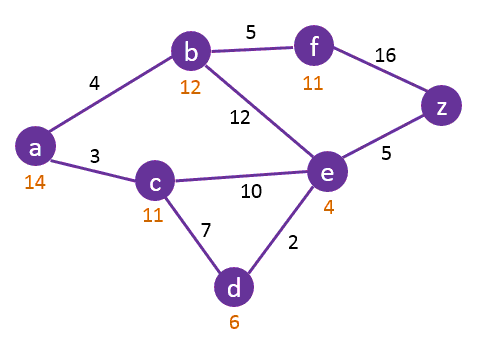
\includegraphics[width=0.5\textwidth]{Figures/AStarExample.png}
  \end{figure}
\end{frame}

\begin{frame}\frametitle{El algoritmo A*}
  \begin{table}
    \begin{tabular}{cccc}
      Paso & Nodo actual & Lista Cerrada & Lista abierta\\
      \hline
      0   & NULL & $\emptyset$          & \{A\}      \\
      1   & A    & \{A\}                & \{B, C\}   \\
      2   & C    & \{A, C\}             & \{B, D, E\}\\
      3   & B    & \{A, C, B\}          & \{D, E, F\}\\
      4   & D    & \{A, C, B, D\}       & \{E, F\}   \\
      5   & $E$  & \{A, C, B, D, E\}    & \{F, Z\}   \\
      6   & $Z$  & \{A, C, B, D, E, Z\} & \{F \}     \\
    \end{tabular}
  \end{table}
  \begin{table}
    \footnotesize
    \begin{tabular}{ccccccc}
      A & B & C & D & E & F & Z \\
      g,f,p & g,f,p & g,f,p & g,f,p & g,f,p & g,f,p & g,f,p\\
      \hline
      0,0,NULL & $\infty,\infty$,NULL & $\infty,\infty$,NULL & $\infty,\infty$,NULL & $\infty,\infty$,NULL & $\infty,\infty$,NULL & $\infty,\infty$,NULL\\
      0,0,NULL & 4, 16, A             & 3, 14, A             & $\infty,\infty$,NULL & $\infty,\infty$,NULL & $\infty,\infty$,NULL & $\infty,\infty$,NULL\\
      0,0,NULL & 4, 16, A             & 3, 14, A             & 10, 16, C            & 13, 17, C            & $\infty,\infty$,NULL & $\infty,\infty$,NULL\\
      0,0,NULL & 4, 16, A             & 3, 14, A             & 10, 16, C            & 13, 17, C            & 9, 20, B             & $\infty,\infty$,NULL\\
      0,0,NULL & 4, 16, A             & 3, 14, A             & 10, 16, C            & \textbf{12, 16, D}   & 9, 20, B             & $\infty,\infty$,NULL\\
      0,0,NULL & 4, 16, A             & 3, 14, A             & 10, 16, C            &         12, 16, D    & 9, 20, B             & 17, 17, E           \\
      0,0,NULL & 4, 16, A             & 3, 14, A             & 10, 16, C            &         12, 16, D    & 9, 20, B             & 17, 17, E           \\
    \end{tabular}
  \end{table}
\end{frame}

\begin{frame}[containsverbatim]\frametitle{Ejercicio 03 - Planeación de rutas}
  Realice lo siguiente:
  \begin{enumerate}
     \item Abra el archivo \texttt{catkin\_ws/src/students/scripts/assignment03a.py} y agregue el siguiente código en la línea 45:
  \begin{lstlisting}[language=Python,firstnumber=45]
for i in range(height):
    for j in range(width):
        if static_map[i,j] > 50:
            for k1 in range(-cost_radius, cost_radius+1):
                for k2 in range(-cost_radius, cost_radius+1):
                    cost = cost_radius - max(abs(k1),abs(k2)) + 1
                    cost_map[i+k1,j+k2] = max(cost, cost_map[i+k1,j+k2])
                  \end{lstlisting}
  \item Corra el simulador con el comando
\begin{verbatim}
    roslaunch bring_up path_planning.launch
\end{verbatim}                  
  \item Corra los nodos de inflado de mapas, mapa de costo y A*, para ello, en tres terminales diferentes, corra los comandos:
\begin{verbatim}
    rosrun students assignment02a.py _inflation_radius:=0.25
    rosrun students assignment03a.py _cost_radius:=0.3
    rosrun students assignment03b.py
\end{verbatim}
  \end{enumerate}
\end{frame}

\begin{frame}\frametitle{Ejercicio 03 - Planeación de rutas}
  \begin{enumerate}
    \setcounter{enumi}{3}
  \item Calcule una ruta utilizando los campos Start Pose y Goal Pose de la GUI:
    \begin{figure}
      \centering
      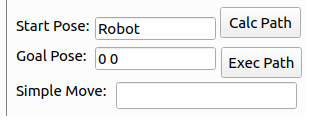
\includegraphics[width=0.35\textwidth]{Figures/GUIPathPlanning.png}
    \end{figure}
  \item Detenga y ejecute de nuevo el inflado de mapas con radios entre 0.1 y 0.5 m y vea qué sucede con el cálculo de rutas.
  \item Detenga y ejecute de nuevo el cálculo del mapa de costo con radios de entre 0.05 y 0.5 m y vea qué sucede con las rutas. 
  \item En el archivo \texttt{assignment03b.py}, cambie la función de distancia de Manhattan por distancia Euclideana, y cambie la conectividad 4 por conectividad 8 (líneas 44, 68 y 69) y vea qué sucede.
  \item Modifique el código para que $h$ sea siempre cero (línea 69) y vea qué sucede con el número de pasos. Pruebe con varias rutas. 
  \end{enumerate}
\end{frame}

\begin{frame}\frametitle{Seguimiento de rutas}
  Hasta el momento ya se tiene una representación del ambiente y una forma de planear rutas. Ahora falta diseñar las leyes de control que hagan que el robot se mueva por la ruta calculada. Este control se hará bajo los siguientes supuestos:
  \begin{itemize}
  \item Se conoce la posición del robot (más adelante se abodará el problema de la localización)
  \item El modelo cinemático es suficiente para modelar el movimiento del robot 
  \item Las dinámicas no modeladas (parte eléctrica y mecánica de los motores) son lo suficientemente rápidas para poder despreciarse
  \end{itemize}
\end{frame}

\begin{frame}\frametitle{Modelo cinemático}
  Considere la base móvil omnidireccional de la figura con configuración $q=(x,y,\theta)$.
  \begin{columns}
    \begin{column}{0.5\textwidth}
      \begin{figure}
        \centering
        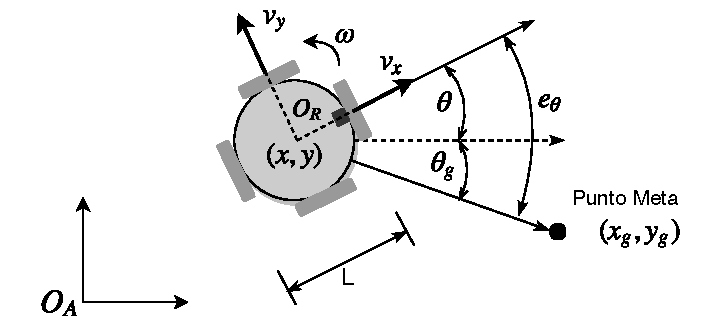
\includegraphics[width=\textwidth]{Figures/GoalPose.pdf}
      \end{figure}
    \end{column}
    \begin{column}{0.5\textwidth}
      El modelo cinemático está dado por
      \begin{eqnarray*} 
        \dot{x} &=& v_x\cos\theta - v_y\sin\theta\label{eq:Kinematic1}\\         
        \dot{y} &=& v_x\sin\theta + v_y\cos\theta\\ 
        \dot{\theta} &=& \omega,\label{eq:Kinematic3}
      \end{eqnarray*}
    \end{column}
  \end{columns}
  \[\]
  \begin{itemize}
  \item $(v_x, v_y, \omega)$ se consideran como señales de control
  \item Corresponden a las velocidades lineales frontal y lateral, y la velocidad angular, con respecto al robot.
  \item La forma de convertir $(v_x, v_y, \omega)$ a velocidades de cada motor varía dependiendo del número de motores y de su posición. 
  \end{itemize}
\end{frame}

\begin{frame}\frametitle{Base omnidireccional de 4 ruedas}
  Dada una base omnidireccional con las ruedas colocadas como se muestra en la figura, las velocidades de cada llanta se pueden obtener como:
  \[\]
  \begin{columns}
    \begin{column}{0.4\textwidth}
      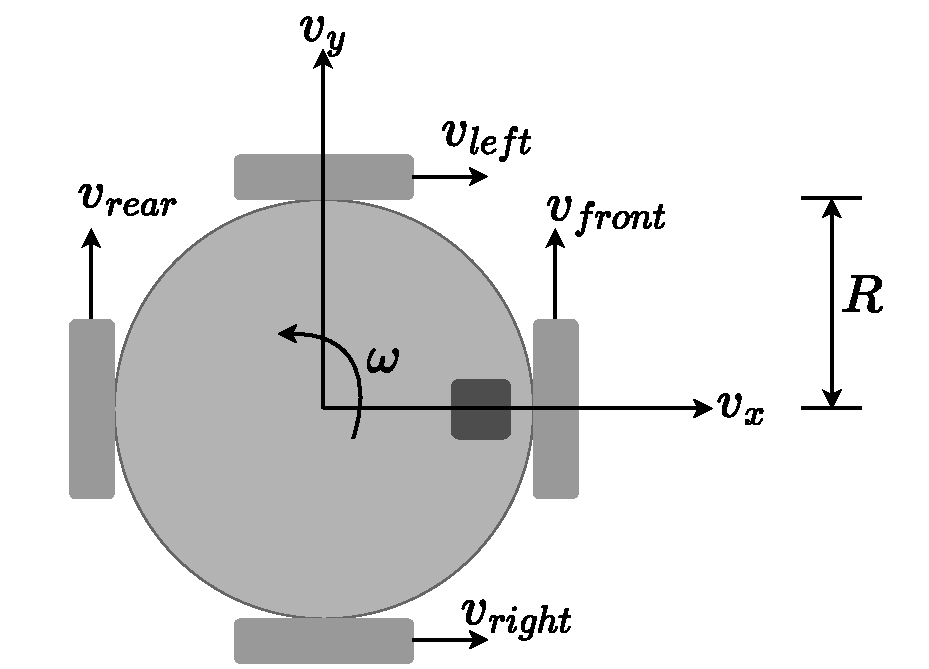
\includegraphics[width=\textwidth]{Figures/Omnidirectional4wheels.pdf}
    \end{column}
    \begin{column}{0.6\textwidth}
      \[\left[\begin{array}{c}
          v_{left}\\v_{right}\\v_{front}\\v_{rear}
              \end{array}\right] =
        \left[\begin{array}{ccc}
                    1 & 0 & -R\\
                    1 & 0 & +R\\
                    0 & 1 & +R\\
                    0 & 1 & -R
        \end{array}\right]
        \left[\begin{array}{c}
           v_{x}\\v_{y}\\ \omega 
        \end{array}\right]
        \]
  \begin{itemize}
  \item Las velocidades de las llantas son lineales.
  \item Para obtener las velocidades angulares, basta con dividir entre el radio de las llantas.
  \end{itemize}
\end{column}
\end{columns}
\[\]
\begin{itemize}
\item Como se puede observar, la matriz anterior no tiene inversa.
\item Se tienen cuatro velocidades de llantas en función de tres variables $(v_x,v_y, \omega)$
\item Esto significa que dadas tres velocidades de llantas, \textbf{la cuarta no puede ser cualquier valor}
\end{itemize}
\end{frame}

\begin{frame}\frametitle{Base omnidireccional de 3 ruedas}
  \begin{itemize}
  \item La base de 4 ruedas omnidireccionales tiene la ventaja de tener mejor tracción y de lograr movimientos rectos más fácilmente.
  \item Tiene la desventaja de que las velocidades pueden indeterminarse si no están bien calculadas.
  \item Una base omnidireccional también puede lograrse con 3 ruedas:
  \end{itemize}
  \begin{columns}
    \begin{column}{0.4\textwidth}
      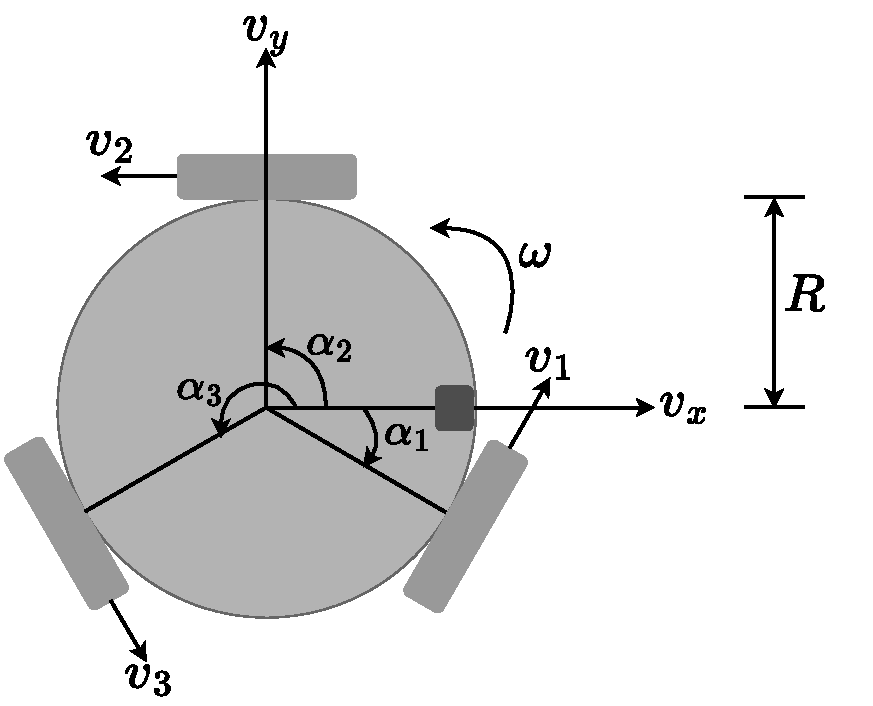
\includegraphics[width=\textwidth]{Figures/Omnidirectional3wheels.pdf}
    \end{column}
    \begin{column}{0.6\textwidth}
      \[\left[\begin{array}{c}
          v_1\\v_2\\v_3
              \end{array}\right] =
        \left[\begin{array}{ccc}
                    -\sin\alpha_1 & \cos\alpha_1 & R\\
                    -\sin\alpha_2 & \cos\alpha_2 & R\\
                    -\sin\alpha_3 & \cos\alpha_3 & R\\
        \end{array}\right]
        \left[\begin{array}{c}
           v_{x}\\v_{y}\\ \omega 
        \end{array}\right]
        \]
\end{column}
\end{columns}
\end{frame}

\begin{frame}\frametitle{Base diferencial}
  \begin{itemize}
  \item Con una base diferencial ya no se tiene movimiento omnidireccional, es decir, se tiene movimiento no holonómico.
  \item El robot ya solo puede tener velocidad frontal $v_x$ pero no velocidad lateral $v_y$.
  \end{itemize}
  \begin{columns}
    \begin{column}{0.4\textwidth}
      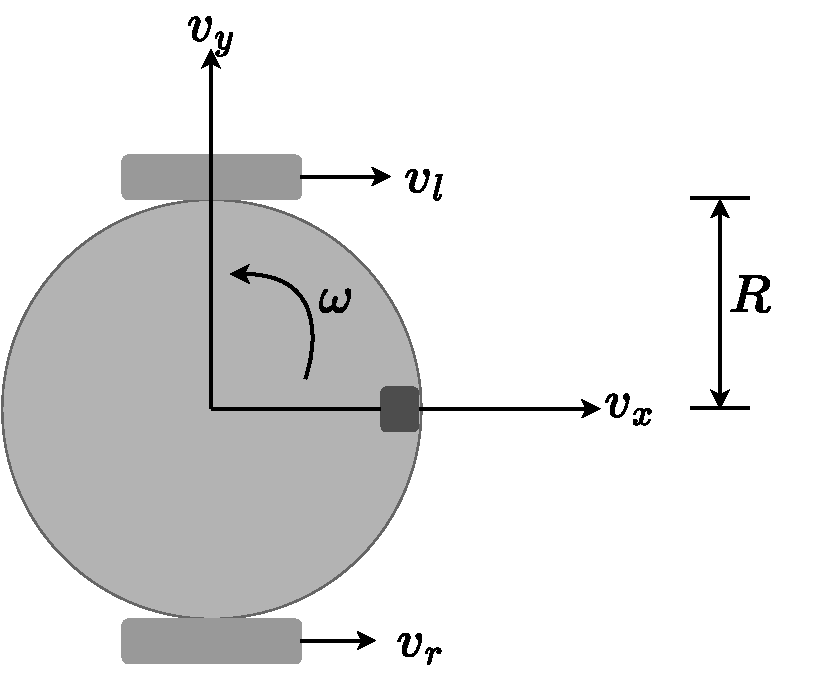
\includegraphics[width=\textwidth]{Figures/DifferentialBase.pdf}
    \end{column}
    \begin{column}{0.6\textwidth}
      \begin{eqnarray*}
        v_l &=& v_x - R\omega\\
        v_r &=& v_x + R\omega
      \end{eqnarray*}
    \end{column}
  \end{columns}
  Esta es la configuración más fácil de lograr debido a la simplicidad del hardware necesario. 
\end{frame}

\begin{frame}\frametitle{Base \textit{Ackermann}}
  \begin{columns}
    \begin{column}{0.7\textwidth}
      \begin{figure}
        \centering
        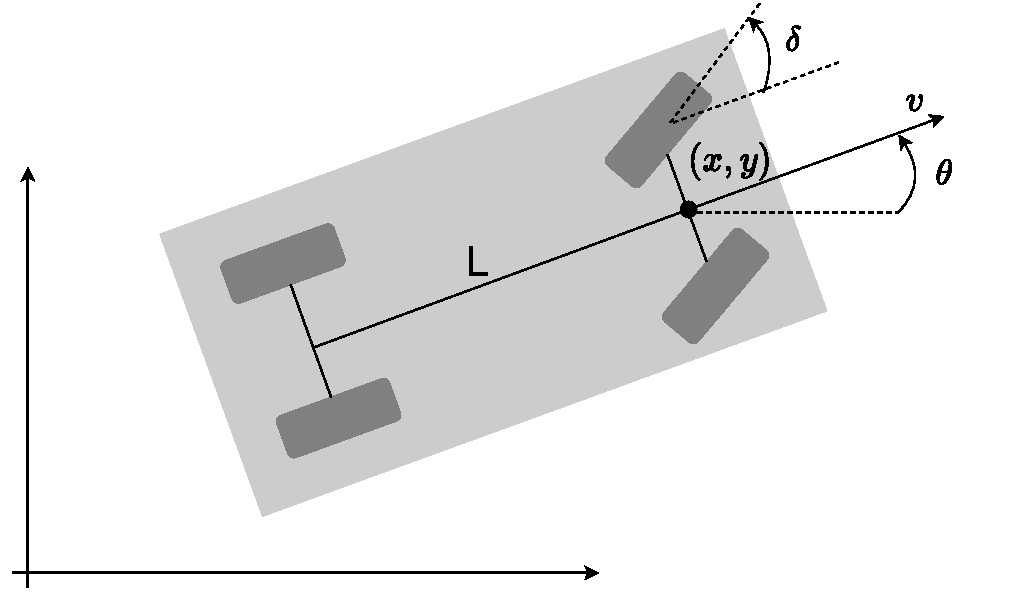
\includegraphics[height=0.5\textheight]{Figures/AckermannBase.pdf}
      \end{figure}
    \end{column}
    \begin{column}{0.3\textwidth}
      \begin{eqnarray*}
        \dot{x} &=& v\cos(\theta + \delta)\\
        \dot{y} &=& v\sin(\theta + \delta)\\
        \dot{\theta} &=& \frac{v}{L}\sin(\delta)
      \end{eqnarray*}
    \end{column}
  \end{columns}
  \begin{itemize}
  \item Es el modelo simplificado de un coche (en un auto real, $\delta$ no es la misma para cada llanta)
  \item Las entradas de control son $(v,\delta)$, es decir, la acción del acelerador y el freno y el ángulo del volante
  \item Las restricciones de movimiento se deben considerar para la planeación de rutas, ya que, por ejemplo, el auto no puede girar sobre su centro. 
  \end{itemize}
\end{frame}

\begin{frame}\frametitle{Control de posición}
  \begin{itemize}
  \item Las leyes de control se diseñarán considerando una base diferencial
  \item Es mejor mover al robot así, pues lo sensores están generalmente al frente
  \end{itemize}
  Si se quiere alcanzar el punto meta $(x_g, y_g)$, las siguientes leyes de control siguientes permiten alcanzar dicho punto meta:
  \begin{eqnarray*}
  v_x    &=& v_{max}e^{-\frac{e_{\theta}^{2}}{\alpha}}\label{eq:Control11}\\
  \omega &=& \omega_{max}\left(\frac{2}{1+e^{-\frac{e_{\theta}}{\beta}}}-1\right)\label{eq:Control12}
  \end{eqnarray*}
  con
  \[e_{\theta} = \atantwo\left(y_g - y, x_g - x\right) - \theta\]
  El error de ángulo $e_\theta$ debe estar siempre en el intervalo $(-\pi, \pi]$. Si la diferencia resulta en un valor fuera de este ángulo, se puede acotar mediante:
  \[e_\theta \leftarrow \left(e_\theta + \pi\right)\% (2\pi) - \pi\]
  donde \% denota el operador módulo (residuo). 
\end{frame}

\begin{frame}\frametitle{Control de posición}
  \begin{itemize}
  \item $v_{max}$ y $\omega_{max}$ son las velocidades linear y angular máximas y dependen de las capacidades físicas del robot.
  \item $\alpha$ y $\beta$ determinan qué tan rápido varían dichas velocidades cuando cambia el error de ángulo.
  \item En general, valores pequeños de $\alpha$ y $\beta$ logran que el robot alcance el punto meta casi en línea recta, sin embargo, valores muy pequeños pueden producir oscilaciones.
  \item Valores grandes de $\alpha$ y $\beta$ producen un movimiento más suave pero pueden hacer que el robot describa curvas muy extensas. 
  \end{itemize}
  \begin{figure}
    \centering
    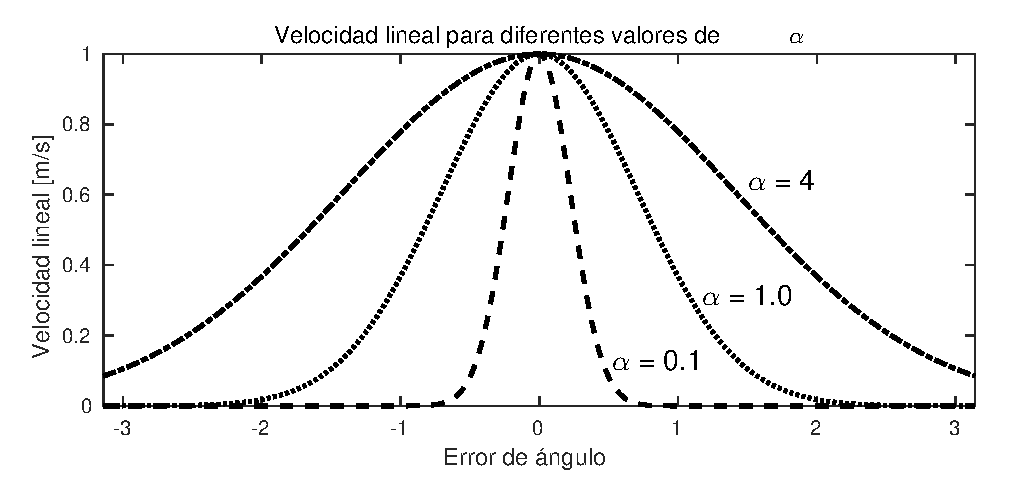
\includegraphics[width=0.45\textwidth]{Figures/LinearSpeed.eps}
    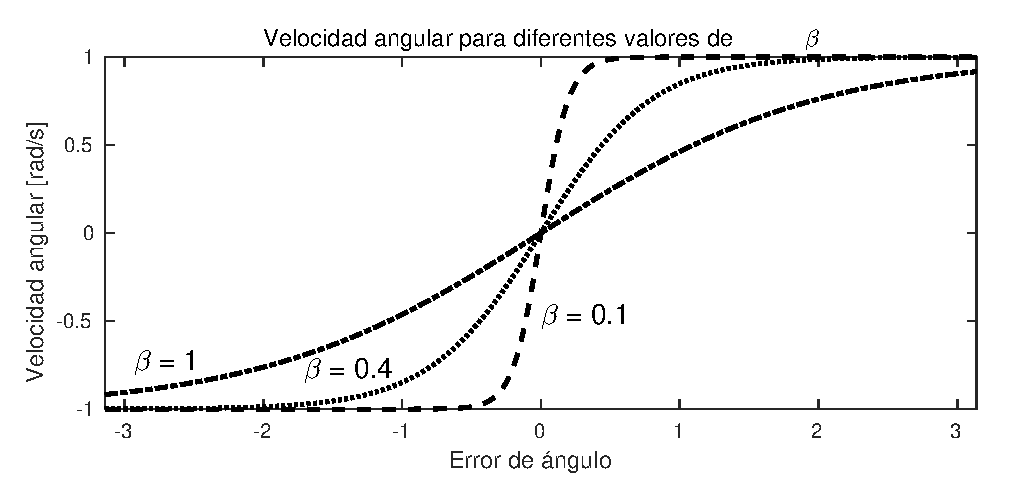
\includegraphics[width=0.45\textwidth]{Figures/AngularSpeed.eps}
  \end{figure}
\end{frame}

\begin{frame}\frametitle{Seguimiento de rutas}
  \begin{itemize}
  \item Hasta el momento se ha planteado cómo alcanzar una posición, pero, ¿para una ruta?
  \item Las rutas son secuencias de puntos. Esta secuencia se podría parametrizar con respecto al tiempo para tener una trayectoria, sin embargo esto resulta muy complicado debido a la complejidad de las rutas.
  \item Una solución más sencilla es aplicar el control de posición para cada punto hasta recorrer toda la ruta.
  \item Las leyes de control solo dependen de $e_\theta$ por lo que el robot no desacelera al acercarse a la meta, provocando fuertes oscilaciones.
  \item Una forma de resolver este problema es ejecutar la ley de control sólo si la distancia al punto meta 

    \[d=\sqrt{(x_g - x_r)^2 + (y_g - y_r)^2}\] 
    
    es mayor que una tolerancia $\epsilon$.
  \item En este caso, el robot se detendrá abruptamente cuando el error de distancia sea menor que $\epsilon$, lo cual tampoco es deseable
  \item Una forma fácil de hacer que el robot acelere y desacelere, o en general, obtener un perfil de velocidad, es mediante el uso de una máquina de estados
    
  \end{itemize}
\end{frame}

\begin{frame}\frametitle{Perfil de velocidad}
  \begin{columns}
    \begin{column}{0.43\textwidth}
      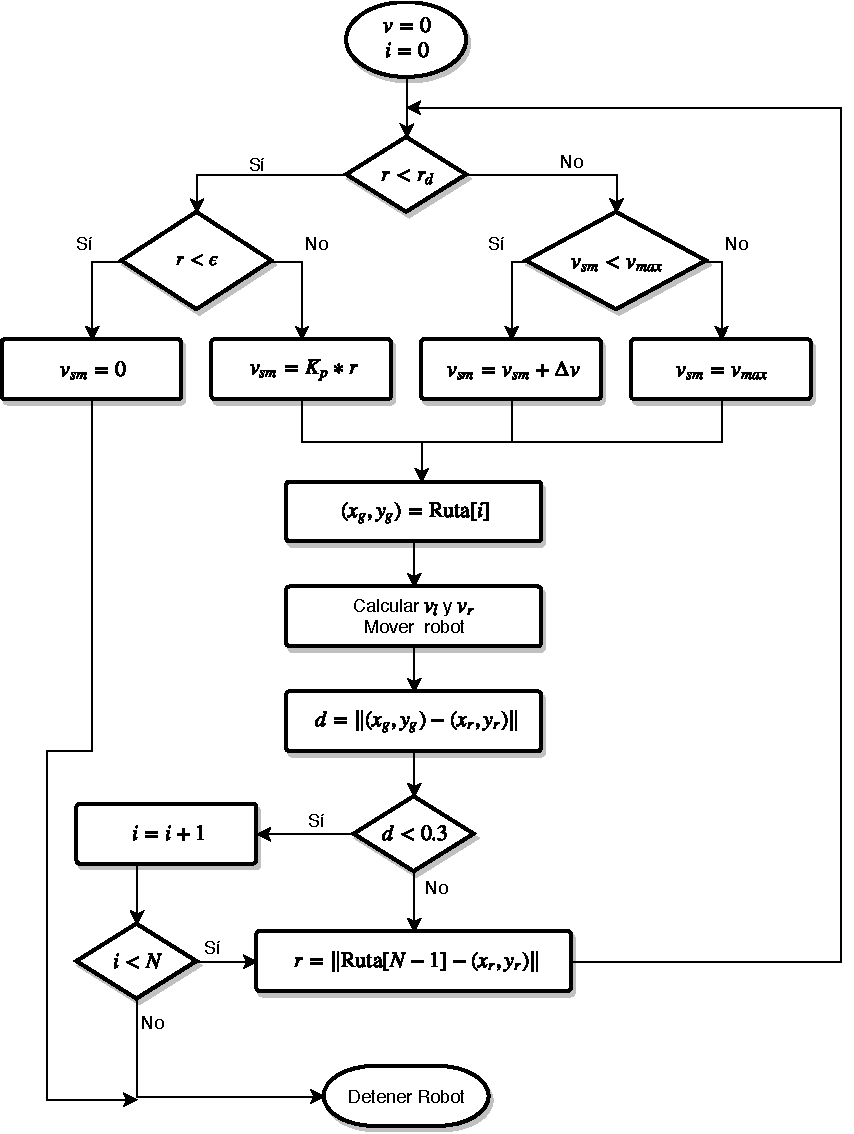
\includegraphics[width=\textwidth]{Figures/AFSM.pdf}
    \end{column}
    \begin{column}{0.5\textwidth}
      Considere una máquina de estados que calcule $v_{max}$ en el control. Sea $v_{sm}$ la nueva velocidad lineal máxima, de modo que ahora se tiene:
      \begin{eqnarray*}
        v      &=& v_{sm}e^{-\frac{e_{\theta}^{2}}{\alpha}}\label{eq:NewControl1}\\
        \omega &=& \omega_{max}\left(\frac{2}{1+e^{-\frac{e_{\theta}}{\beta}}}-1\right)\label{eq:NewControl2}
      \end{eqnarray*}
      con
      \begin{itemize}
      \item $r$: Distancia a la meta global
      \item $\epsilon$: Distancia a la que se considera que el robot alcanzó la meta global
      \item $r_d$: Distancia a la meta global para desacelerar
      \item $\Delta v$: Aceleración 
      \end{itemize}
    \end{column}
  \end{columns}
\end{frame}

\begin{frame}\frametitle{Perfil de velocidad}
  La siguiente figura muestra un ejemplo de una ruta y las velocidades lineales generadas usando solo las leyes de control (izquierda) y usando la máquina de estados para un perfil de velocidad (derecha). 
  \begin{figure}
    \centering
    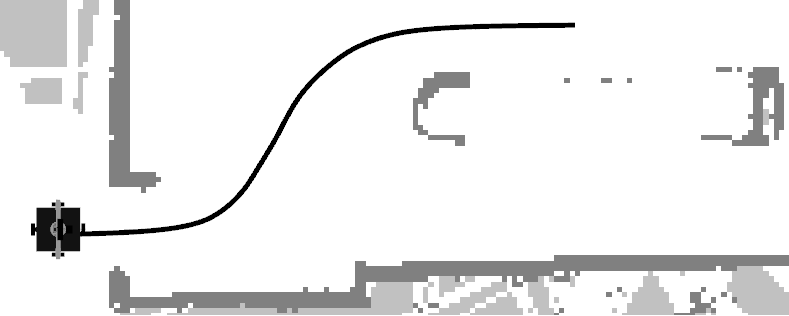
\includegraphics[width=0.45\textwidth]{Figures/SpeedProfilePath.png}
  \end{figure}
  \begin{figure}
    \centering
    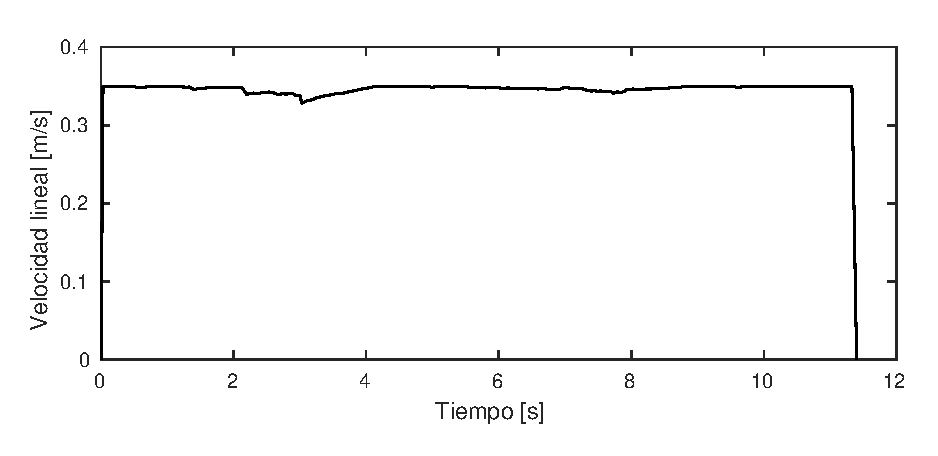
\includegraphics[width=0.45\textwidth]{Figures/SpeedWithoutProfile.eps}
    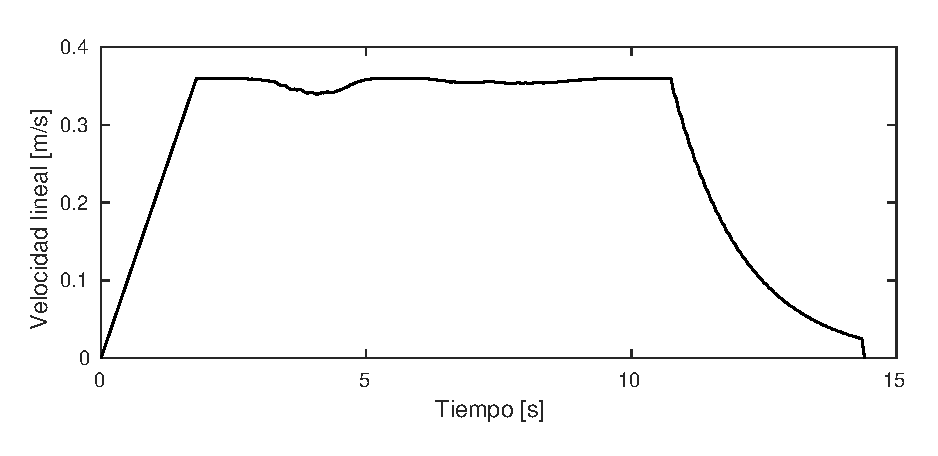
\includegraphics[width=0.45\textwidth]{Figures/SpeedWithProfile.eps}
  \end{figure}
\end{frame}

\begin{frame}[containsverbatim]\frametitle{Ejercicio 04 - Seguimiento de rutas}
  Realice lo siguiente:
  \begin{enumerate}
  \item Abra el archivo \texttt{catkin\_ws/src/students/scripts/assignment04.py} y agregue el siguiente código en la línea 45 para implementar las leyes de control:
    \begin{lstlisting}[language=Python,firstnumber=45]
    v_max = 0.5
    w_max = 1.0
    alpha = 0.1
    beta  = 0.1
    error_a = math.atan2(goal_y - robot_y, goal_x - robot_x) - robot_a
    error_a = (error_a + math.pi)%(2*math.pi) - math.pi 
    cmd_vel.linear.x  = v_max*math.exp(-error_a*error_a/alpha)
    cmd_vel.angular.z = w_max*(2/(1 + math.exp(-error_a/beta)) - 1)
  \end{lstlisting}
  \item Ejecute la simulación igual que en los ejercicios anteriores. 
  \item Ejecute el inflado de obstáculos, mapa de costo, algoritmo A* y seguimiento de rutas (\texttt{assignment02a.py, assignment03a.py, assignment03b.py} y \texttt{assignment04.py})
  \item Con el botón \textit{2D Nav Goal} del visualizador \textit{RViz}, selecccione un punto meta en el mapa y observe qué sucede. 
  \item Pruebe con diferentes valores de $\alpha$ y $\beta$ hasta obtener un movimiento satisfactorio. 
  \end{enumerate}
\end{frame}


\begin{frame}\frametitle{Suavizado de rutas}
  \begin{itemize}
  \item Puesto que las rutas se calcularon a partir de celdas de ocupación, están compuestas de esquinas.
  \item La esquinas no son deseables, pues suelen generar cambios bruscos en las señales de control.
  \item La ruta verde de la imagen es una muestra de una ruta calculada por A*.
  \item Es preferible una ruta como la azul. 
  \end{itemize}
  \begin{figure}
    \centering
    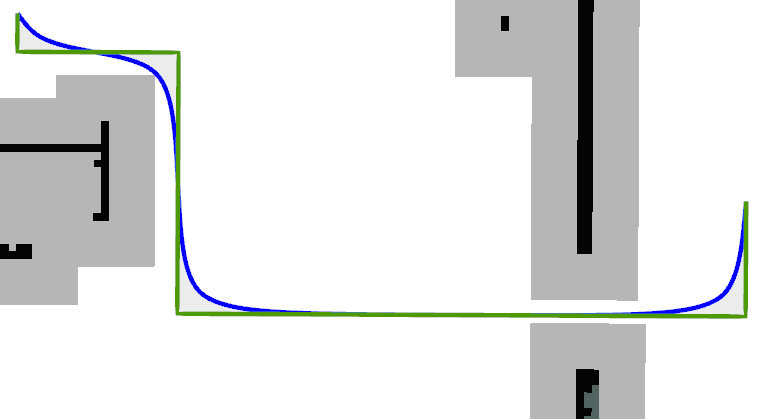
\includegraphics[height=0.45\textheight]{Figures/PathSmoothingExample.png}
  \end{figure}
  Existen varias formas de suavizar la ruta generada:
  \begin{itemize}
  \item Splines
  \item Descenso del gradiente
  \end{itemize}
\end{frame}

\begin{frame}\frametitle{Suavizado mediante splines}
  \begin{itemize}
  \item Un \textit{spline} es una función definida a tramos por polinomios.
  \item La forma más común son los splines de tercer grado o \textit{cubic splines}
  \item Se ajusta un polinomio de tercer grado por cada par de puntos
  \item La derivada al final de un tramo debe ser igual a la derivada al inicio del siguiente tramo.
  \item Aplicando estas condiciones para cada par 
  \end{itemize}
  
\end{frame}


\begin{frame}\frametitle{Suavizado mediante descenso del gradiente}
  Otra forma de suavizar la ruta es planteando una función de costo y encontrando el mínimo. Los puntos negros representan la ruta de A* compuesta por los puntos $Q=\{q_0, q_1, \dots, q_n\}$ y los puntos azules representan una ruta suave $P=\{p_0, p_1,\dots, p_n\}$.
  \begin{columns}
    \begin{column}{0.5\textwidth}
      \begin{figure}
        \centering
        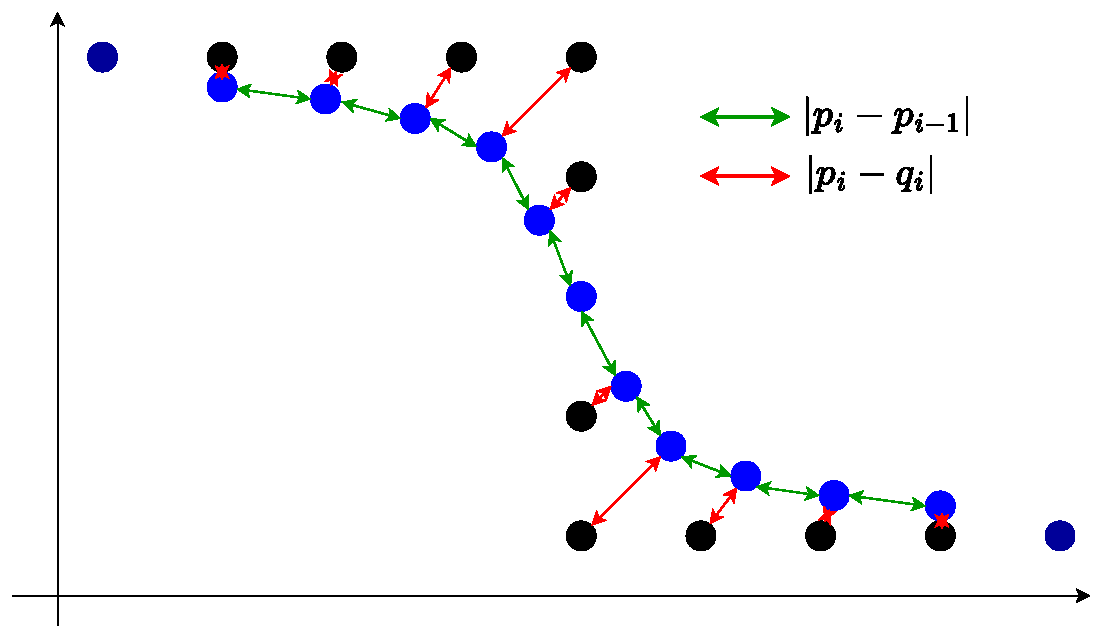
\includegraphics[width=\textwidth]{Figures/PathSmoothing.pdf}
      \end{figure}
    \end{column}
    \begin{column}{0.5\textwidth}
      Considere la función de costo:
      \[J = \alpha\frac{1}{2}\sum_{i=1}^{n-1}\left(p_i - p_{i-1}\right)^2 + \beta\frac{1}{2}\sum_{i=1}^{n-1}(p_i - q_i)^2\]
      \begin{itemize}
      \item $J$ es la suma de distancias entre un punto y otro de la ruta suavizada, y entre la ruta suavizada y la original.
      \item Si la ruta es muy suave, $J$ es grande.
      \item Si la ruta es muy parecida a la original, $J$ también es grande.
      \item Una ruta ni muy suave ni muy parecida a la original, logrará minimizar $J$.
      \end{itemize}
    \end{column}
  \end{columns}
\end{frame}

\begin{frame}\frametitle{Suavizado mediante descenso del gradiente}
  \begin{itemize}
  \item Una forma de encontrar el mínimo es resolviendo $\nabla J(p) = 0$, y luego evaluando la matriz Hessiana para determinar si el punto crítico $p_c$ es un mínimo.
  \item Esto se puede complicar debido al alto número de variables en $p$.
  \item Una forma más sencilla, es mediante el descenso del gradiente.
  \end{itemize}
  \begin{columns}
    \begin{column}{0.7\textwidth}
  \begin{algorithm}[H]
    \footnotesize
  \DontPrintSemicolon
  \KwData {Función $J(p):\mathbb{R}^n\rightarrow \mathbb{R}$ a minimizar}
  \KwResult{Vector $p$ que minimiza la función $J$}
  $p\leftarrow p_{init}$ //Fijar una estimación inicial\;
  \While{$|\nabla J(p)| > tol$}
  {
    $p \leftarrow p - \epsilon \nabla J (p)$ //$p$ se modifica un poco en sentido contrario al gradiente.\;
  }
  Devolver $p$
  \caption{Descenso del gradiente}
\end{algorithm}
\end{column}
\end{columns}
\[\]
El descenso del gradiente devuelve el mínimo local más cercano a la condición inicial $p_0$. Pero la función de costo $J$ tiene solo un mínimo global. El gradiente de la función de costo $J$ se calcula como:
  \[\underbrace{\left[\frac{}{}\alpha(p_0 - p_1)+\beta(p_0 - q_0)\right. }_{\dfrac{\partial J}{\partial p_0}}
,\dots ,
\underbrace{\frac{}{}\alpha(2p_i - p_{i-1} - p_{i+1})+\beta(p_i - q_i)}_{\dfrac{\partial J}{\partial p_i}}
,\dots ,
\underbrace{\left.\alpha(p_{n-1} - p_{n-2})+\beta(p_{n-1}-q_{n-1})\frac{}{}\right]}_{\dfrac{\partial J}{\partial p_{n-1}}}
\]
\end{frame}

\begin{frame}\frametitle{Suavizado mediante descenso del gradiente}
  
  Para no variar los puntos inicial y final de la ruta, la primer y última componentes de $\nabla J$ se dejarán en cero. El algoritmo de descenso del gradiente queda como:
  \[\]
\begin{algorithm}[H]
\DontPrintSemicolon
  \DontPrintSemicolon
  \KwData{Conjunto de puntos $Q = \{q_0\dots q_i \dots q_{n-1}\}$ de la ruta original, parámetros $\alpha$ y $\beta$, ganancia $\epsilon$ y tolerancia $tol$\;}
  \KwResult{Conjunto de puntos $P = \{p_0\dots p_i \dots p_{n-1}\}$ de la ruta suavizada\;}
  $P \leftarrow Q$\;
  $\nabla J_0 \leftarrow 0$\;
  $\nabla J_{n-1} \leftarrow 0$\;   
  \While{ $\Vert\nabla J(p_i)\Vert > tol$}
  {
    \ForEach{$i \in [1,n-1)$}
    {
      $\nabla J_i \leftarrow \alpha (2p_i - p_{i-1} - p_{i+1}) + \beta (p_i - q_i)$\;
    }
    $P \leftarrow P - \epsilon \nabla J$
  }
  regresar $P$
  \caption{Suavizado de rutas mediante descenso del gradiente}
\end{algorithm}
\end{frame}

\begin{frame}[containsverbatim]\frametitle{Ejercicio 05 - Suavizado y seguimiento de rutas}
  Realice lo siguiente:
  \begin{enumerate}
     \item Abra el archivo \texttt{catkin\_ws/src/students/scripts/assignment05.py} y agregue el siguiente código en la línea 39:
  \begin{lstlisting}[language=Python,firstnumber=39]
nabla[0], nabla[-1] = 0, 0
while numpy.linalg.norm(nabla) > tol*len(P) and steps < 100000:
    for i in range(1, len(Q)-1):
       nabla[i] =alpha*(2*P[i] - P[i-1] - P[i+1]) + beta*(P[i] - Q[i])
    P = P - epsilon*nabla
    steps += 1
  \end{lstlisting}
  \item Corra la simulación igual en los ejercicios anteriores anteriores. 
  \item Corra los nodos de inflado de mapas, mapa de costo, A* y seguimiento de rutas.
  \item Corra el suavizado de rutas mediante el comando:
    \begin{verbatim}
  rosrun students assignment05.py _alpha:=0.9 _beta:=0.1
\end{verbatim}
  \item En el visualizador, observe la diferencia entre la ruta original calculada con A* (en azul) y la ruta suavizada (en verde). 
  \end{enumerate}
\end{frame}


\begin{frame}[containsverbatim]\frametitle{Ejercicio 05 - Suavizado y seguimiento de rutas}
  \begin{enumerate}
    \setcounter{enumi}{5}
  \item Detenga el suavizado de rutas y vuelva a ejecutar con diferentes valores de $\alpha$ y $\beta$.
  \item Detenga el suavizado de rutas y sintonice las constantes $\alpha$ y $\beta$ del control de posición (ejercicio 04) hasta que el robot siga muy de cerca la ruta calculada (no importa que tenga cambios abruptos de velocidad).
  \item Ejecute el suavizado de rutas y el control de posición con las constantes sintonizadas.
  \end{enumerate}
\end{frame}

\section{Evasión de obstáculos}
\begin{frame}\frametitle{Evasión de obstáculos}
  \begin{itemize}
  \item Hasta el momento se tiene una manera de representar el ambiente, planear una ruta y seguirla
  \item ¿Qué pasa si en el ambiente hay un obstáculo que no estaba en el mapa?
  \item Se requiere de una técnica reactiva para evadir obstáculos
  \item Una posible solución es el uso de campos potenciales artificiales
  \end{itemize}
\end{frame}

\begin{frame}\frametitle{Campos potenciales artificiales}
  El objetivo de esta técnica es diseñar una función $U(q):\mathbb{R}^n\rightarrow \mathbb{R}$ que represente energía potencial.
  \begin{itemize}
  \item El gradiente $\nabla U(q) = \left[\frac{\partial U}{\partial q_1},\dots,\frac{\partial U}{\partial q_n}\right]$ es una fuerza.
  \item Se debe diseñar de modo que tenga un mínimo global en el punto meta y máximos locales en cada obstáculo.
  \item Si el robot se mueve siempre en sentido contrario al gradiente $\nabla U$ llegará al punto meta siguiendo una ruta alejada de los obstáculos.
  \item Ha varias formas de diseñar la función $U(q)$, algunas son:
    \begin{itemize}
    \item Algoritmo \textit{wavefront}, requiere una discretización del espacio (requiere mapa previo), pero no presenta mínimos locales.
    \item Campos atractivos y repulsivos, no requieren mapa previo, pero pueden presentar mínimos locales. 
    \end{itemize}
  \end{itemize}
\end{frame}

\begin{frame}\frametitle{Potenciales atractivos y repulsivos}
  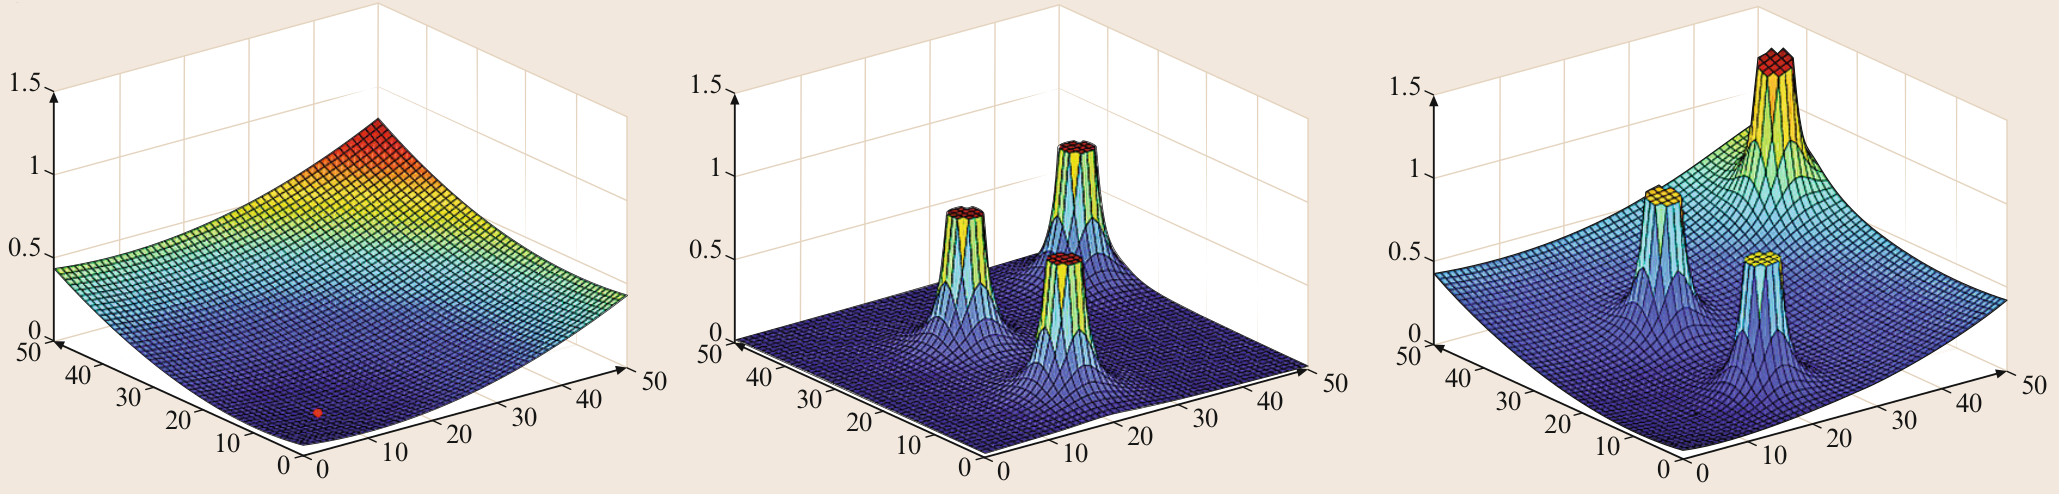
\includegraphics[width=\textwidth]{Figures/PotFieldsExample.png}
  \begin{itemize}
  \item \textbf{Campos repulsivos:} Por cada obstáculo se diseña una función $U_{rej_i}(q)$ con un máximo local en la posición $q_{o_i}$ del obstáculo.
  \item \textbf{Campo atractivo:} Se diseña una función $U_{att}(q)$ con un mínimo global en el punto meta $q_g$.
  \item La función potencial total $U(q)$ se calcula como
    \[ U(q) = U_{att}(q) + \frac{1}{N}\sum_{i=1}^N U_{rej_i}(q)\]
  \end{itemize}
\end{frame}

\begin{frame}\frametitle{Fuerzas atractiva y repulsivas}
  Puesto que el gradiente es un operador lineal, se pueden diseñar directamente las fuerzas atractiva $F_{att}(q) = \nabla U_{att}(q)$ y repulsivas $F_{rej_i}(q) = \nabla U_{rej_i}(q)$, de modo que la fuerza total será:
  \[ \nabla U(q) = F(q) = F_{att}(q) + \frac{1}{N}\sum_{i=1}^N F_{rej_i}(q)\]
  Una propuesta de estas fuerzas es:
  \begin{eqnarray*}
    \label{eq:attractive}
    F_{att} &=& \zeta \dfrac{\left(q - q_g\right) }{\Vert q - q_g \Vert},\qquad \zeta > 0\label{eq:PotFieldsAttraction}\\
    F_{rej} &=& \begin{cases}
                  \eta\left(\sqrt{\dfrac{1}{d} - \dfrac{1}{d_0}}\right)\dfrac{q_{o_i} - q}{d}
                  & \quad\textrm{si}\quad d < d_0\\
                  0 & \quad\textrm{en otro caso}
                \end{cases}
  \end{eqnarray*}
  donde
  \begin{itemize}
  \item $q=(x,y)$ es la posición del robot
  \item $q_g=(x_g, y_g)$ es el punto que se desea alcanzar
  \item $q_{o_i} = (x_{o_i}, y_{o_i})$ es la posición del $i$-ésimo obstáculo
  \item $d_0$ es una distancia de influencia. Más allá de $d_0$ los obstáculos no producen efecto alguno
  \item $\zeta$ y $\eta$, junto con $d_0$, son constantes de sintonización
  \end{itemize}
\end{frame}


\begin{frame}\frametitle{Evasión de obstáculos por campos potenciales}
  \begin{itemize}
  \item Aunque las ecuaciones anteriores suponen que se conoce la posición de cada obstáculo $q_{o_i}$, en realidad ésta aparece siempre en la diferencia $q_{o_i} - q$, es decir, solo se requiere su posición relativa al robot.
  \item Los campos potenciales se implementan utilizando el lidar, donde cada lectura se considera un obstáculo. 
  \end{itemize}
  \begin{figure}
    \centering
    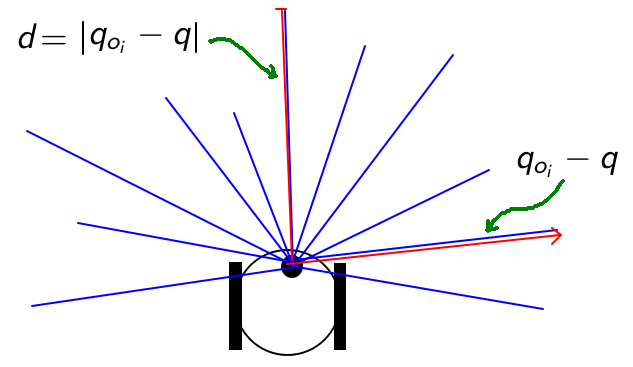
\includegraphics[width=0.4\textwidth]{Figures/PotFieldsLidar.png}
  \end{figure}
  Las lecturas del lídar generalmente son pares distancia-ángulo $(d_i,\theta_i)$ expresados con respecto al robot, por lo que, si se conoce la posición del robot $(x_r,y_r,\theta_r)$, la posición de cada obstáculo se puede calcular como:
  \begin{eqnarray*}
    x_{oi} &=& x_r + d_i\cos(\theta_i + \theta_r)\\
    y_{oi} &=& y_r + d_i\sin(\theta_i + \theta_r)\\
  \end{eqnarray*}
\end{frame}

\begin{frame}\frametitle{Evasión de obstáculos por campos potenciales}
  Finalmente, para que el robot alcance el punto de menor potencial, se puede emplear el descenso del gradiente:
  \[\]
  \begin{algorithm}[H]
  \DontPrintSemicolon
  \KwData{Posición inicial $q_s$, posición meta $q_g$, posiciones $q_{oi}$ de los obstáculos y tolerancia $tol$}
  \KwResult{Secuencia de puntos $\{q_0,q_1, q_2, \dots\}$ para evadir obstáculos y alcanzar el punto meta}
  \;
$q \leftarrow q_s$\;
\While{$\Vert\nabla U(q)\Vert > tol$}
{
  $q \leftarrow q - \epsilon F(q)$\;
  $[v,\omega] \leftarrow $ leyes de control con $q$ como posición deseada\;
}
  \caption{Descenso del gradiente para mover al robot a través de un campo potencial.}
  \label{alg:PotFields}
\end{algorithm}
\end{frame}

\begin{frame}\frametitle{Evasión de obstáculos por campos potenciales}
  Ejemplo de movimiento:
  \begin{figure}
    \centering
    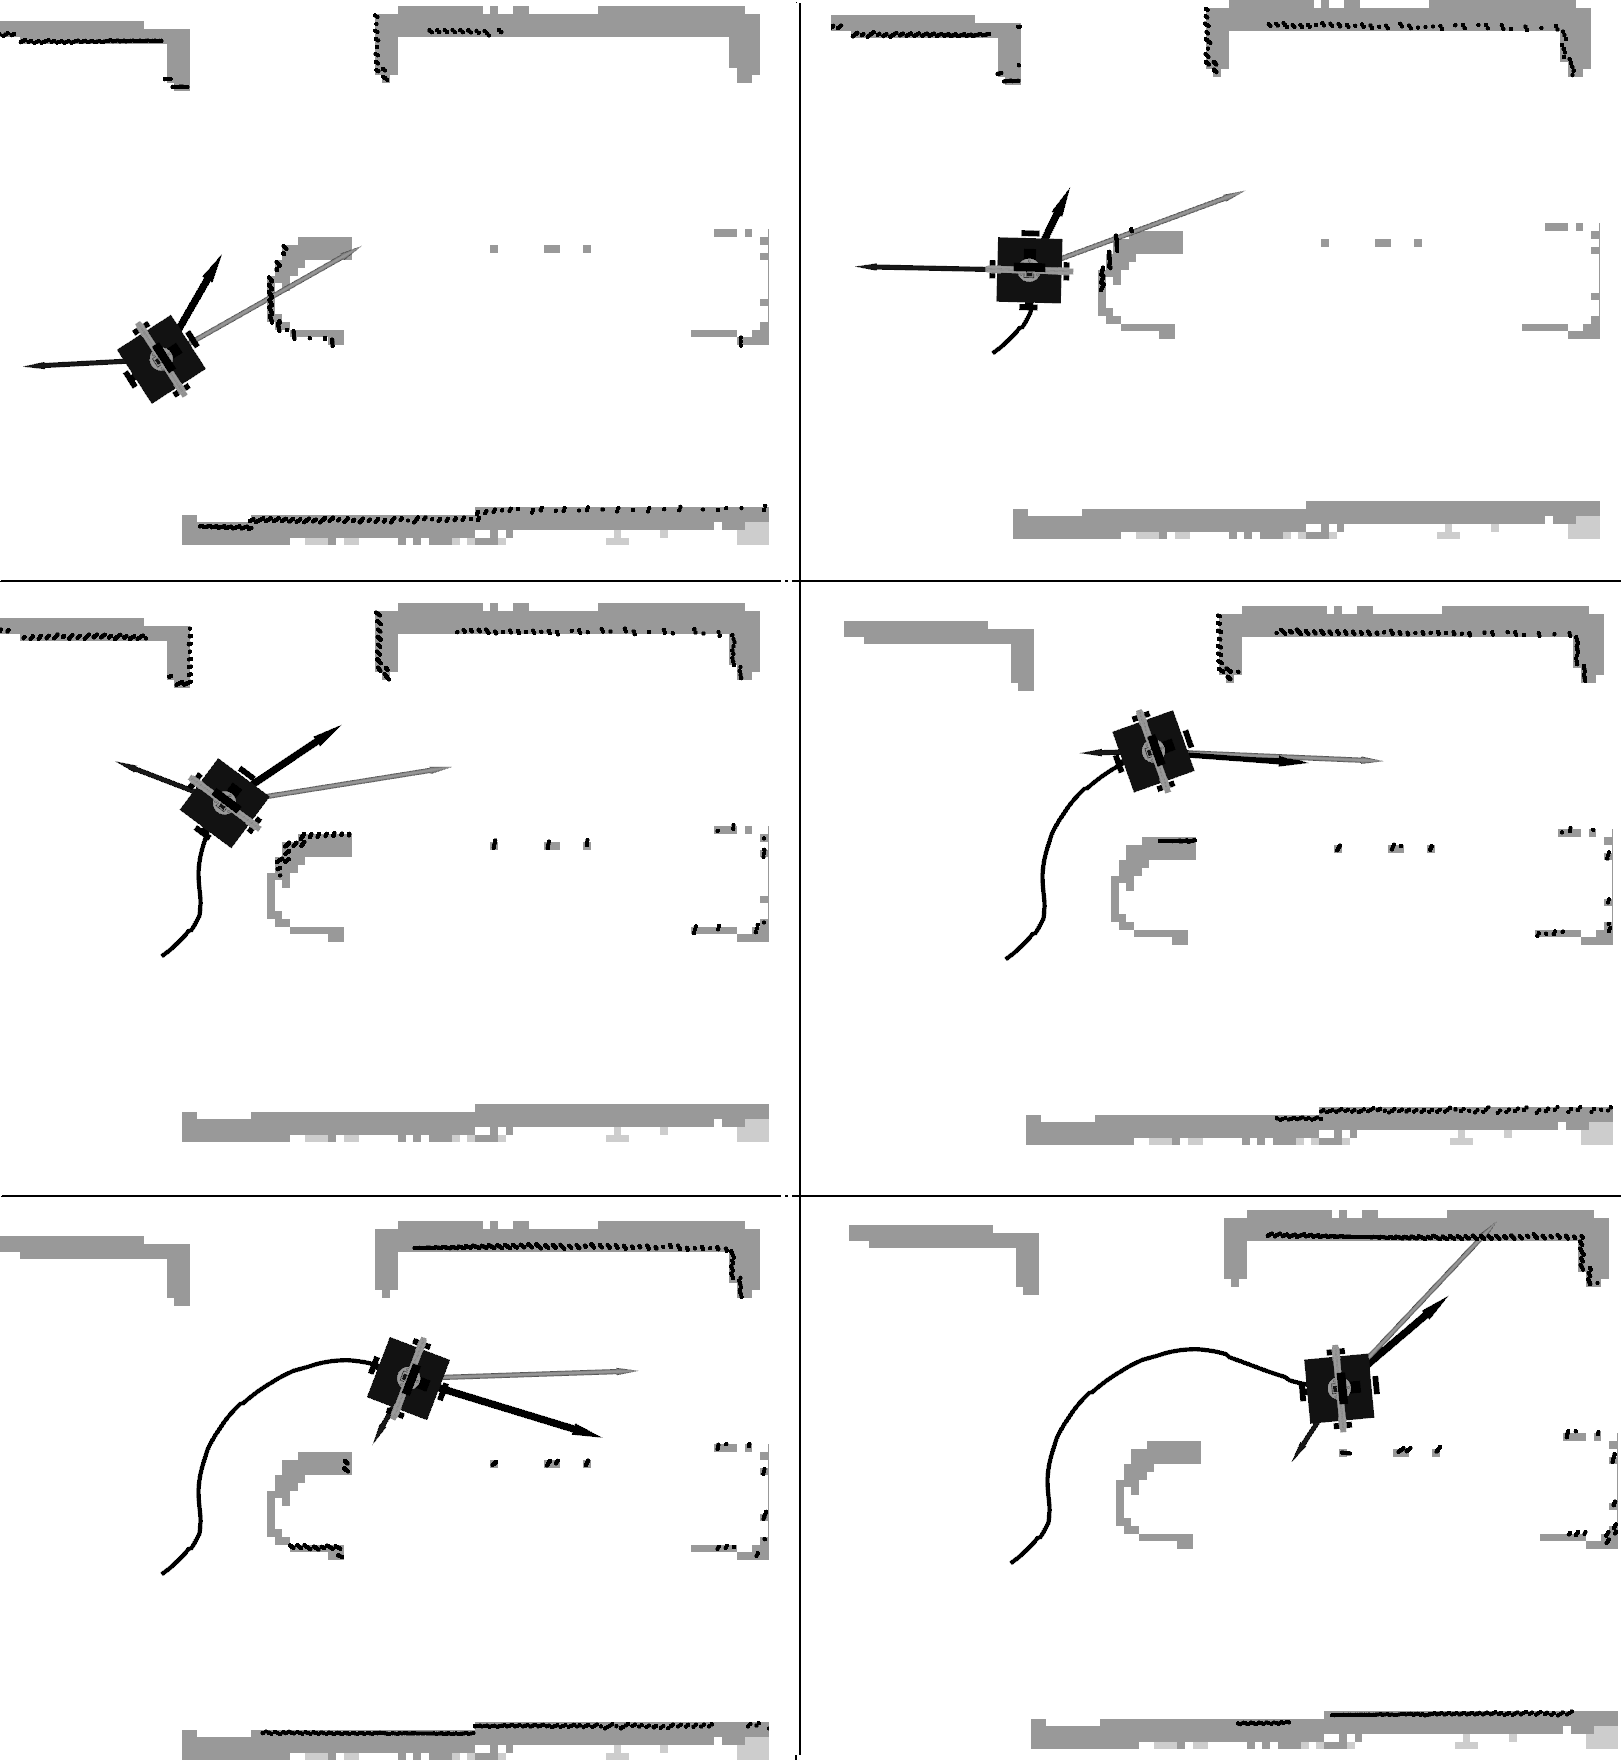
\includegraphics[height=0.85\textheight]{Figures/PotFieldsExecution.png}
  \end{figure}
\end{frame}

\begin{frame}[containsverbatim]\frametitle{Ejercicio 06 - Evasión de obstáculos}
  \begin{enumerate}
  \item Abra el archivo \texttt{catkin\_ws/src/students/scripts/assignment06.py} y realice lo siguiente:
    \begin{enumerate}
    \item En la función \texttt{calculate\_control} implemente el control utilizado en el ejercicio 04 (copy-paste)
    \item Implemente el cálculo de la fuerza atractiva en la función \texttt{attraction\_force}:
      \begin{lstlisting}[language=Python,firstnumber=65]
zeta = 1.0
force_x, force_y = robot_x - goal_x, robot_y - goal_y
mag = math.sqrt(force_x**2 + force_y**2)
return [zeta*force_x/mag, zeta*force_y/mag] if mag != 0 else [0,0]
\end{lstlisting}
    \item En la función \texttt{rejection\_force}, implemente el cálculo de la fuerza repulsiva total
      \[F_{rej} = \frac{1}{N}\sum_{i=1}^N F_{rej_i}(q)\]
      Considere que dada lectura del láser es un obstáculo, como se explicó anteriormente:
      \begin{lstlisting}[language=Python,firstnumber=65]
d0  = 1.0
eta = 4.0  
[force_x, force_y] = [0,0]
for [d,theta] in laser_readings:
    mag = 0 if d >= d0 or d <= 0 else eta*math.sqrt(1/d - 1/d0)
    force_x += mag*math.cos(robot_a + theta)
    force_y += mag*math.sin(robot_a + theta)
return [force_x/len(laser_readings), force_y/len(laser_readings)]
  \end{lstlisting}
\end{enumerate}
\end{enumerate}
\end{frame}

\begin{frame}[containsverbatim]\frametitle{Ejercicio 06 - Evasión de obstáculos}
  \begin{enumerate}    
\setcounter{enumi}{7}
  \item Ejecute la simulación con el comando
    \begin{verbatim}
   roslaunch surge_et_ambula obstacle_avoidance.launch
\end{verbatim}
  \item Ejecute la evasión por campos potenciales mediante el comando
\begin{verbatim}
   rosrun students assignment06.py
\end{verbatim}
  \item Con la opción \textit{2D Nav Goal} del visualizador \textit{RViz}, selecccione un punto meta en el mapa.
  \item Observe qué sucede.
  \item Pruebe con diferentes constantes de sintonización y observer los cambios en el comportamiento. 
  \end{enumerate}
\end{frame}


\begin{frame}\frametitle{Localización}
  El problema de la localización consiste en determinar la configuración $q$ del robot dada un mapa y un conjunto de lecturas de los sensores.
  \begin{itemize}
  \item La localización se podría lograr simplemente integrando los comandos de velocidad del robot.
  \item Si se conoce perfectamente la configuración inicial y el robot ejecuta perfectamente los comandos de movimiento, entonces la simple integración de la velocidad de los motores sería suficiente.
  \item Esto por supuesto no es posible. Se tiene incertidumbre tanto en la estimación inicial de la posición como en la ejecución de cada movimiento.
  \item Es decir, el robot pierde información sobre su posición en cada movimiento. 
  \end{itemize}
\end{frame}

\section{Localización}

\begin{frame}\frametitle{Localización}
  Existen principalmente dos tipos:
\[\]
  \begin{columns}
    \begin{column}{0.5\textwidth}
      \textbf{Localización local: }
      \begin{itemize}
      \item Requiere una estimación inicial \textit{cercana} a la posición real del robot, de otro modo, no converge.
      \item Suele ser menos costosa computacionalmente.
      \item Un método común es el Filtro de Kalman Extendido.
      \end{itemize}
    \end{column}
    \begin{column}{0.5\textwidth}
      \textbf{Localización global:}
      \begin{itemize}
      \item La estimación inicial puede ser cualquiera.
      \item Suele ser computacionalmente costosa.
      \item Un método común son los Filtros de Partículas. 
      \end{itemize}
      \[\]
      \[\]
    \end{column}
  \end{columns}
\end{frame}

\begin{frame}\frametitle{Localización probabilística}
  \begin{itemize}
  \item En la localización probabilística, en lugar de llevar una sola hipótesis sobre la posición del robot, se mantiene una \textit{distribución de probabilidad} sobre todo el espacio de hipótesis.
  \item El enfoque probabilístico permite manejar las incertidumbres inherentes al movimiento y al sensado.
  \item El reto es obtener una distribución de densidad de probabilidad (PDF) sobre todas las posibles posiciones del robot.
  \item En general, los métodos probabilísticos de estimación se componen de dos pasos:
    \begin{enumerate}
    \item \textbf{Predicción:} Se modifica la PDF de la posición del robot con base en los comandos y el modelo de movimiento.
    \item \textbf{Actualización:} Se corrige la predicción mezclando la información de PDF predicha con información de los sensores. Se obtiene una PDF de la posición y se repite el proceso. 
    \end{enumerate}
  \end{itemize}
  
\end{frame}

\begin{frame}\frametitle{El Filtro de Kalman Extendido}
  \begin{figure}
    \centering
    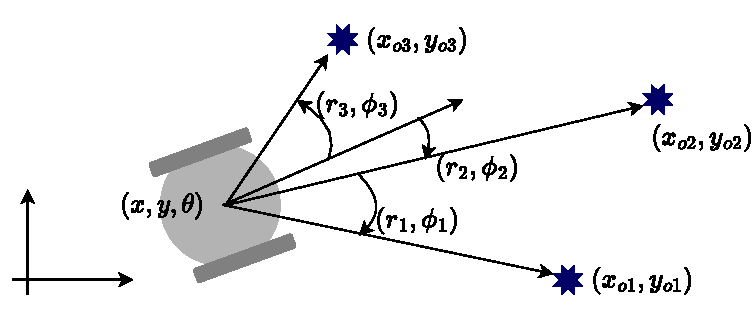
\includegraphics[height=0.4\textheight]{Figures/EKF1.pdf}
  \end{figure}
  \begin{columns}
    \begin{column}{0.45\textwidth}
      Modelo de transición de estados:
      \[\left.
      \begin{array}{cclc}
        x_{k+1}      &=& x_k + (\Delta t)v\cos(\theta_k) & + n_{p1}\\
        y_{k+1}      &=& y_k + (\Delta t)v\sin(\theta_k) & + n_{p2}\\
        \theta_{k+1} &=& \theta_k + (\Delta t)\omega     & + n_{p3}
      \end{array}\right\}f(x)
    \]
    donde $n_p\in\mathbb{R}^3$ es ruido de proceso que es distribuye normalmente con
    media cero y matriz de covarianza conocida $Q\in\mathbb{R}^{3\times 3}$
    \end{column}
    \begin{column}{0.55\textwidth}
      Modelo de observación:
      \[\left.
        \begin{array}{cclc}
                 &\vdots& & \\
        r_{i}    &=& \sqrt{(x_k - x_{oi})^2 + (y_k - y_{oi})^2}   & + n_{m1}\\
        \phi_{i} &=& atan2(y_k - y_{oi}, x_k - x_{oi}) - \theta_k & + n_{m2}\\
                 &\vdots& & \\
      \end{array}\right\}h(x)
    \]
    donde $M$ es el número de marcas observadas, $n_m\in\mathbb{R}^{2M}$ es ruido de medición que se distribuye normalmente con media cero y matriz de covarianza conocida $R\in\mathbb{R}^{2M\times 2M}$
    \end{column}
  \end{columns}
\end{frame}

\begin{frame}\frametitle{Algoritmo de estimación del EKF}
  \begin{figure}
    \centering
    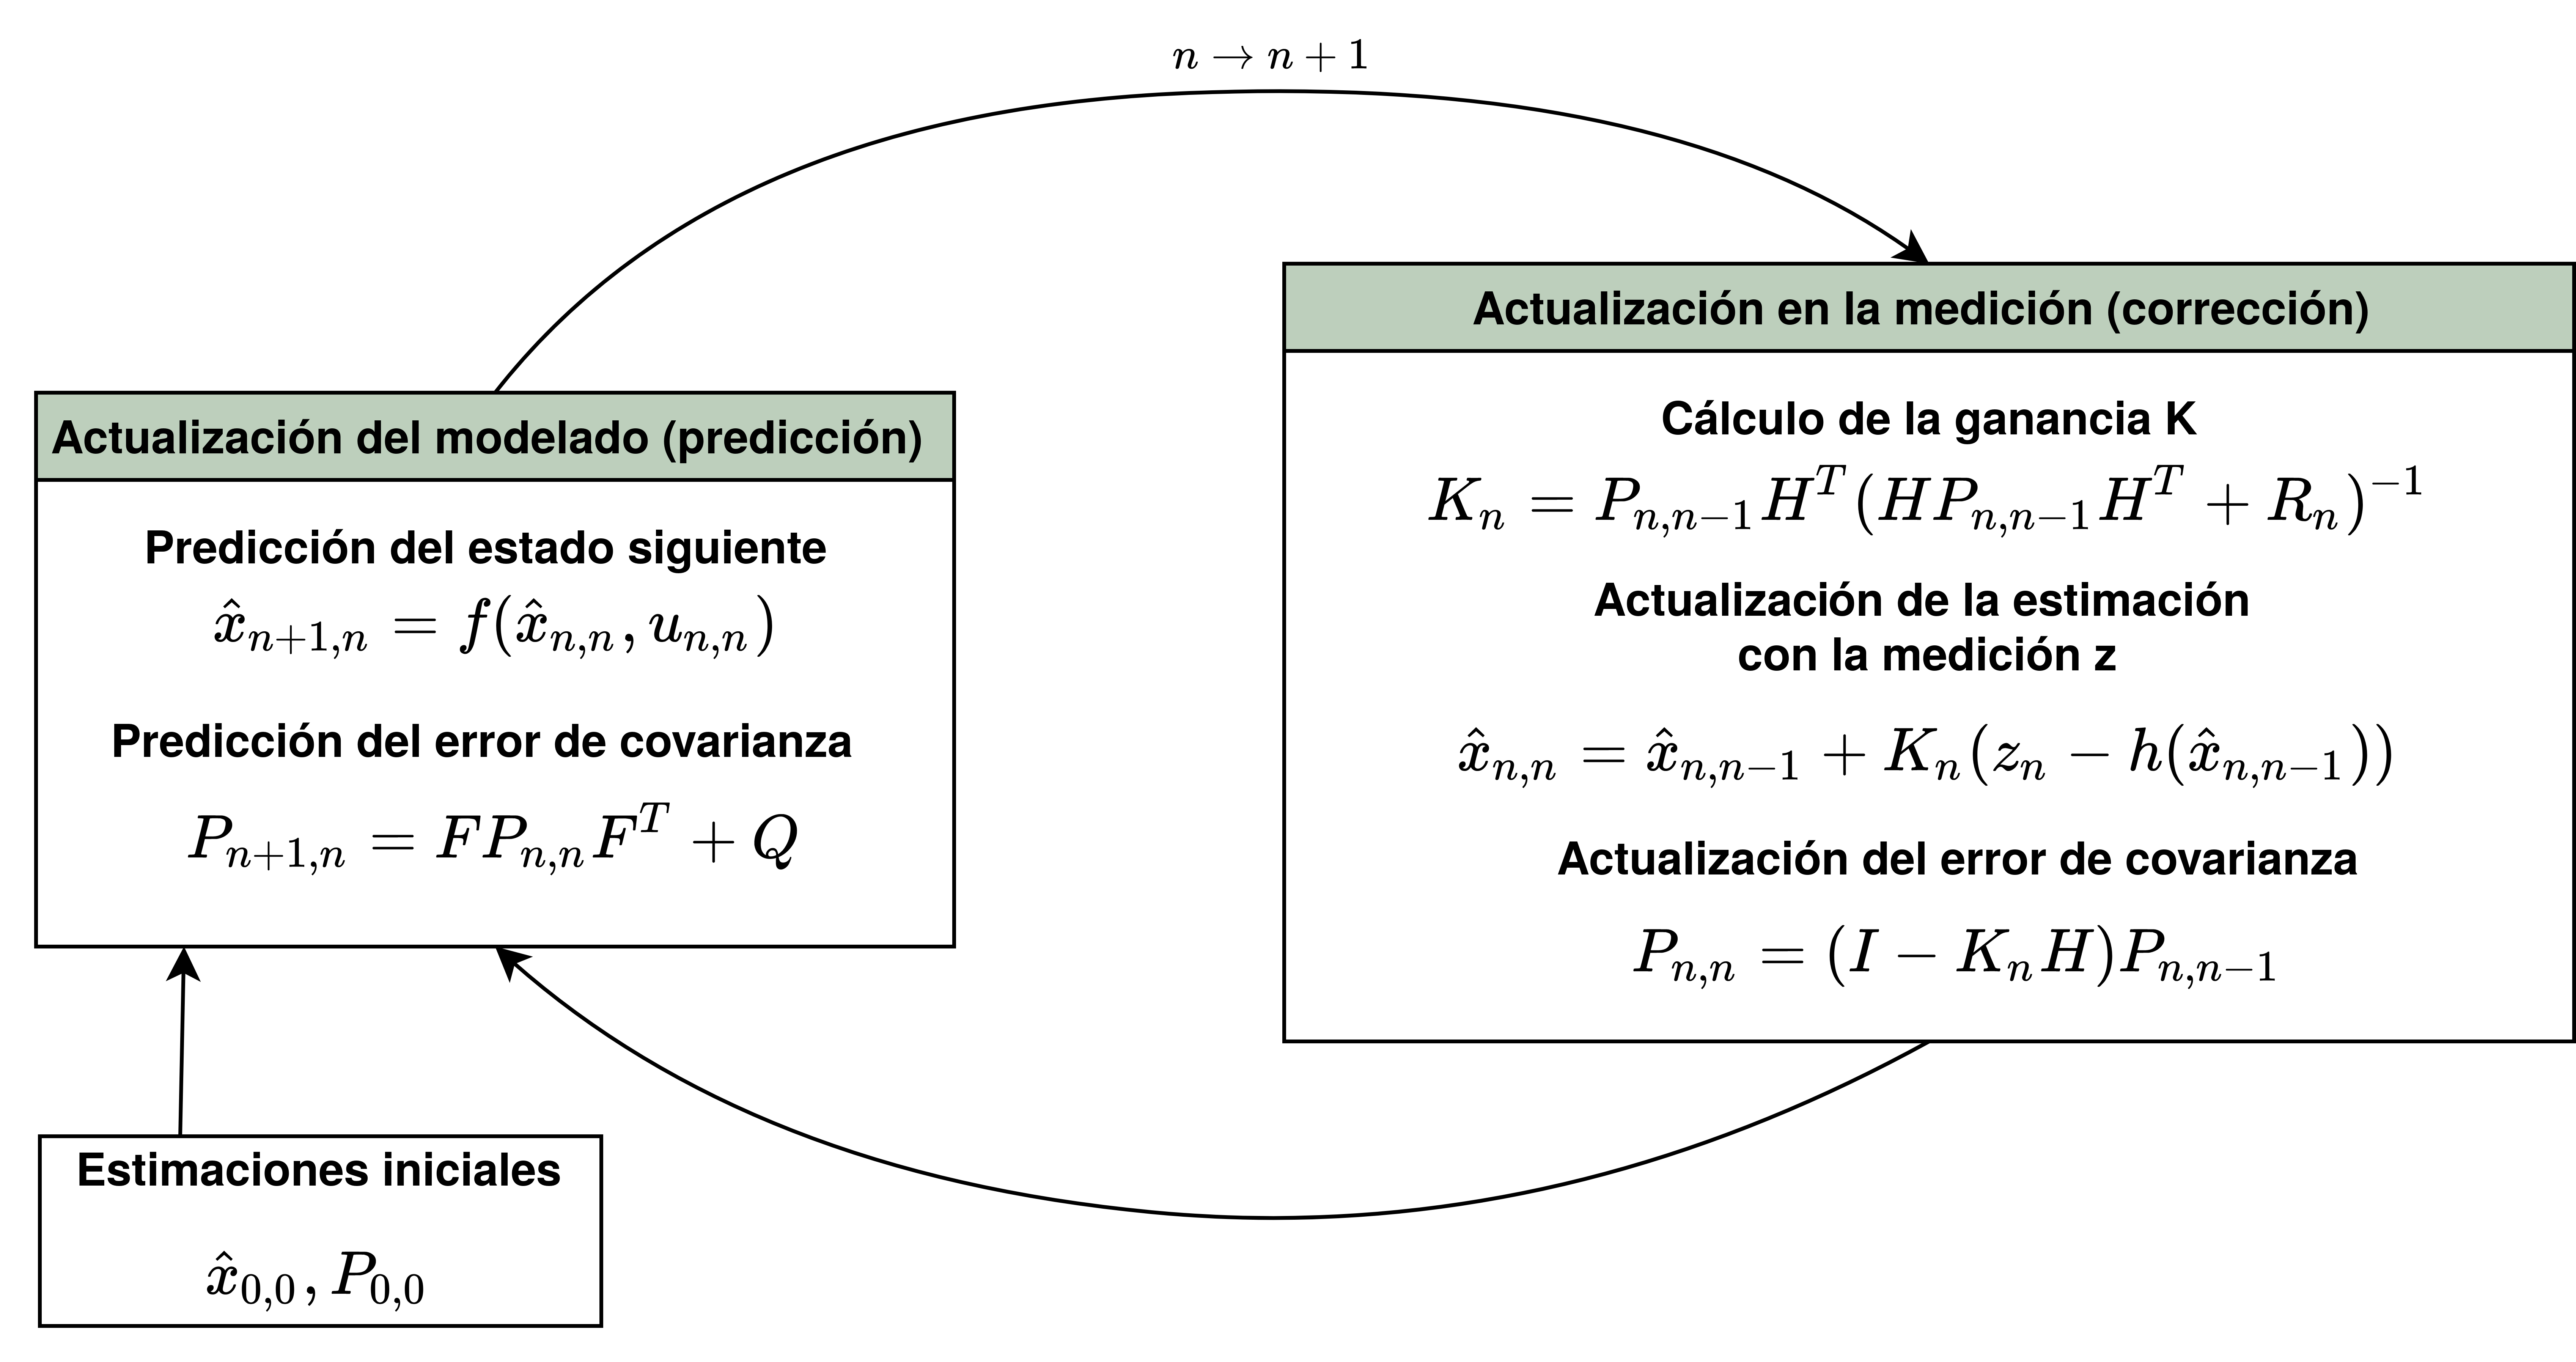
\includegraphics[height=0.6\textheight]{Figures/EKF2.png}
  \end{figure}
  con:
  \begin{itemize}
  \item $P$ : Matriz de covarianza del error de estimación
  \item $F$ : Jacobiano de $f(x)$
  \item $H$ : Jacobiano de $h(x)$
  \end{itemize}
\end{frame}

\begin{frame}\frametitle{El EKF como un filtro Bayesiano}
  \begin{itemize}
  \item El EKF obtiene una distribución de probabilidad \textit{a posteriori} $P(A|B)$: la probabilidad de que el robot esté en una posición dadas las lecturas de los sensores.
  \item El modelo de observación representa la verosimilitud $P(B|A)$: la probabilidad de obtener ciertas lecturas dado un cierto estado del robot.
  \item La estimación dada por $\hat{x}_{k+1}$ es la distribución a priori $P(A)$
  \item EKF supone una distribución normal, es decir $\hat{x}_{k+1}$ es una variable aleatoria que se distribuye normalmente con media en $f(x_k, u_k)$ y covarianza $Q$
  \end{itemize}
\end{frame}

\begin{frame}\frametitle{Filtros de partículas}
  \begin{itemize}
  \item A diferencia del EKF que supone una distribución normal, los filtros de partículas suponen una distribución no paramétrica.
  \item Se consideran $N$ suposiciones de la posición del robot. A cada suposición $(x,y,\theta)$ se le llama partícula. 
  \item La distribución \textit{a priori} se calcula realizando simulaciones de movimiento para cada partícula.
  \item El modelo de observación también se realiza mediante simulaciones de los sensores para cada partículas.
  \item Para obtener la distribución \textit{a posteriori} se comparan las lecturas simuladas con la lectura del sensor real y se realiza un muestreo aleatorio con reemplazo. Cada partícula tiene una probabilidad de ser muestreada, proporcional a la similitud de su lectura simulada con el sensor real.
  \end{itemize}
\end{frame}

\begin{frame}\frametitle{Filtros de Partículas}
  \begin{figure}
    \centering
    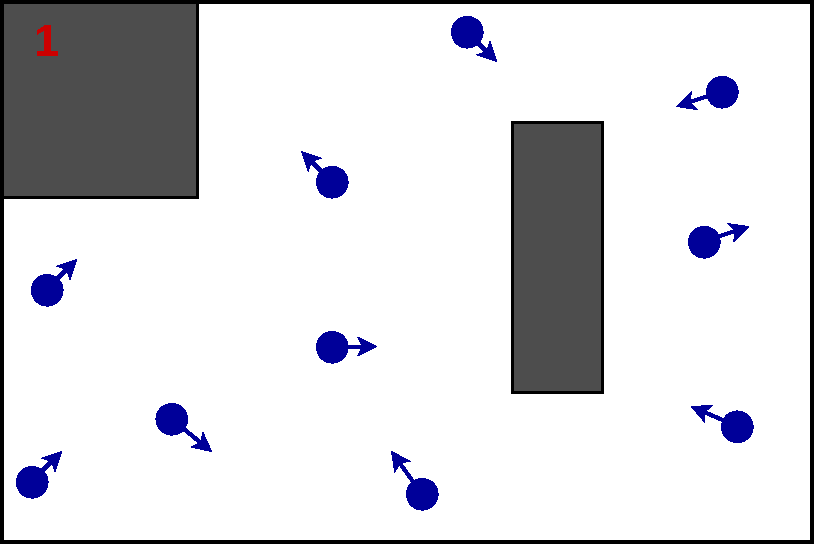
\includegraphics[width=0.6\textwidth]{Figures/ParticleFilter1.pdf}
  \end{figure}
\end{frame}

\begin{frame}\frametitle{Simulación del sensor}
\end{frame}

\begin{frame}\frametitle{Comparación de simulación con real}
\end{frame}

\begin{frame}\frametitle{Remuestreo con reemplazo}
\end{frame}

\begin{frame}\frametitle{Desplazamiento de partículas}
\end{frame}

\begin{frame}[containsverbatim]\frametitle{Ejercicio 07 - Localización por filtros de partículas}
Realice lo siguiente:
  \begin{enumerate}
  \item Abra el archivo \texttt{catkin\_ws/src/students/src/assignment07.cpp} y realice lo siguiente:
    \begin{enumerate}
    \item En la función \texttt{get\_initial\_distribution} genere $N$ partículas con pose $(x,y,\theta)$ aleatoria con distribución uniforme. 
    \item Complete la función \texttt{simulate\_particle\_scans} para generar lecturas del láser simuladas dado un mapa y la posición de las partículas. 
    \item En la función \texttt{calculate\_particle\_similarities}, calcule la similitud vista en clase para cada partícula y normalice los valores para sumen 1.
    \item Complete la función \texttt{random\_choice} para devolver un índice aleatorio $i$ dada una distribución de probabilidad cualquiera determinada por un arreglo de probabilidades $p$.
    \item En la función \texttt{resample\_particles} implemente el remuestreo con reemplazo visto en clase, dado un conjunto de partículas y una distribución de probabilidad.
    \item En la función \texttt{move\_particles} implemente el movimiento de partículas dado un desplazamiento.
    \item Complete la función \texttt{main} de acuerdo con las instrucciones dadas en los comentarios del código. 
    \end{enumerate}
  \item Compile el código con el comando \texttt{catkin\_make} (el directorio de trabajo debe ser \texttt{catkin\_ws})
  \item Ejecute la simulación con el comando \texttt{roslaunch bring\_up localization.launch}
  \item Corra la práctica con el comando \texttt{rosrun students assignment07}
  \item Mueva el robot con la GUI y observe lo que sucede en el visualizador. 
  \item El código debe recompilarse con cada cambio. 
  \end{enumerate}
\end{frame}

